%%%%%%%%%%%%%%%%%%%%%%%%%%%%%%%%%%%%%%%%%%%%%%%%%%%%%%%%%%%%%%%%%%%%%%%%%%%%%%%
%                       CARREGA DE LA CLASSE DE DOCUMENT                      %
%                                                                             %
% Les opcions admissibles son:                                                %
%      12pt / 11pt            (cos dels tipus de lletra; no feu servir 10pt)  %
%                                                                             %
% catalan/spanish/english     (llengua principal del treball)                 %
%                                                                             % 
% french/italian/german...    (si necessiteu fer servir alguna altra llengua) %
%                                                                             %
% listoffigures               (El document inclou un Index de figures)        %
% listoftables                (El document inclou un Index de taules)         %
% listofquadres               (El document inclou un Index de quadres)        %
% listofalgorithms            (El document inclou un Index d'algorismes)      %
%                                                                             %
%%%%%%%%%%%%%%%%%%%%%%%%%%%%%%%%%%%%%%%%%%%%%%%%%%%%%%%%%%%%%%%%%%%%%%%%%%%%%%%

\documentclass[11pt,spanish,listoffigures,listoftables]{tfgetsinf}


\usepackage{pgfplotstable} % Para leer y mostrar tablas desde CSV
\usepackage{booktabs}       % Para mejorar el diseño de la tabla
\usepackage{multirow}       % Para fusionar filas
\usepackage{caption}
\usepackage{subcaption}

\usepackage[acronym]{glossaries} % Para crear un glosario

\usepackage{float}          % Para usar [H] en las figuras
\usepackage{amsmath}        % Para usar \text en modo matemático
\usepackage{tabularx}       % Para usar el entorno tabularx
\usepackage{array}          % Para usar >{} en las columnas de la tabla
%%%%%%%%%%%%%%%%%%%%%%%%%%%%%%%%%%%%%%%%%%%%%%%%%%%%%%%%%%%%%%%%%%%%%%%%%%%%%%%
%                     CODIFICACIO DEL FITXER FONT                             %
%                                                                             %
%    windows fa servir normalment 'ansinew'                                   %
%    amb linux es possible que siga 'latin1' o 'latin9'                       %
%    Pero el mes recomanable es fer servir utf8 (unicode 8)                   %
%                                          (si el vostre editor ho permet)    % 
%%%%%%%%%%%%%%%%%%%%%%%%%%%%%%%%%%%%%%%%%%%%%%%%%%%%%%%%%%%%%%%%%%%%%%%%%%%%%%%

\usepackage[utf8]{inputenc} 
%%%%%%%%%%%%%%%%%%%%%%%%%%%%%%%%%%%%%%%%%%%%%%%%%%%%%%%%%%%%%%%%%%%%%
% Para conseguir que la tabla de contenido no salga en rojo
%%%%%%%%%%%%%%%%%%%%%%%%%%%%%%%%%%%%%%%%%%%%%%%%%%%%%%%%%%%%%%%%%%%%%

\hypersetup{ colorlinks=true, linkcolor=black, urlcolor=cyan, }


\newacronym{ai}{AI}{Artificial Intelligence}



%%%%%%%%%%%%%%%%%%%%%%%%%%%%%%%%%%%%%%%%%%%%%%%%%%%%%%%%%%%%%%%%%%%%%%%%%%%%%%%
%                        ALTRES PAQUETS I DEFINICIONS                         %
%                                                                             %
% Carregueu aci els paquets que necessiteu i declareu les comandes i entorns  %
%                                          (aquesta seccio pot ser buida)     %
%%%%%%%%%%%%%%%%%%%%%%%%%%%%%%%%%%%%%%%%%%%%%%%%%%%%%%%%%%%%%%%%%%%%%%%%%%%%%%%



%%%%%%%%%%%%%%%%%%%%%%%%%%%%%%%%%%%%%%%%%%%%%%%%%%%%%%%%%%%%%%%%%%%%%%%%%%%%%%%
%                        DADES DEL TREBALL                                    %
%                                                                             %
% titol, alumne, tutor i curs academic                                        %
%%%%%%%%%%%%%%%%%%%%%%%%%%%%%%%%%%%%%%%%%%%%%%%%%%%%%%%%%%%%%%%%%%%%%%%%%%%%%%%

\title{Detección de defectos en objetos en movimiento mediante Redes Neuronales Convolucionales con optimizaciones específicas para hardware NVIDIA}
\author{Haro Armero, Abel}
\tutor{Flich Cardo, José \\
López Rodríguez, Pedro Juan}
\curs{2024-2025}

%%%%%%%%%%%%%%%%%%%%%%%%%%%%%%%%%%%%%%%%%%%%%%%%%%%%%%%%%%%%%%%%%%%%%%%%%%%%%%%
%                     PARAULES CLAU/PALABRAS CLAVE/KEY WORDS                  %
%                                                                             %
% Independentment de la llengua del treball, s'hi han d'incloure              %
% les paraules clau i el resum en els tres idiomes                            %
%%%%%%%%%%%%%%%%%%%%%%%%%%%%%%%%%%%%%%%%%%%%%%%%%%%%%%%%%%%%%%%%%%%%%%%%%%%%%%%

\keywords{Xarxes Neuronals Convolucionals, Detecció de defectes, Visió per computador, NVIDIA Jetson, Temps real, Optimització energètica}
   {Redes Neuronales Convolucionales, Detección de defectos, Visión por computador, NVIDIA Jetson, Tiempo real, Optimización energética}
   {Convolutional Neural Networks, Defect Detection, Computer Vision, NVIDIA Jetson, Real-Time, Energy Optimization}

%%%%%%%%%%%%%%%%%%%%%%%%%%%%%%%%%%%%%%%%%%%%%%%%%%%%%%%%%%%%%%%%%%%%%%%%%%%%%%%
%                              INICI DEL DOCUMENT                             %
%%%%%%%%%%%%%%%%%%%%%%%%%%%%%%%%%%%%%%%%%%%%%%%%%%%%%%%%%%%%%%%%%%%%%%%%%%%%%%%

\begin{document}

%%%%%%%%%%%%%%%%%%%%%%%%%%%%%%%%%%%%%%%%%%%%%%%%%%%%%%%%%%%%%%%%%%%%%%%%%%%%%%%
%              RESUMS DEL TFG EN VALENCIA, CASTELLA I ANGLES                  %
%%%%%%%%%%%%%%%%%%%%%%%%%%%%%%%%%%%%%%%%%%%%%%%%%%%%%%%%%%%%%%%%%%%%%%%%%%%%%%%

\begin{abstract}
Aquest treball de fi de grau aborda el desafiament de la detecció automàtica de defectes en objectes que es desplacen en entorns industrials, com ara línies de producció. Es presenta el disseny i la implementació d'un sistema complet de visió artificial basat en tècniques d'aprenentatge profund.

El nucli del sistema és un model de xarxa neuronal convolucional (CNN), específicament una variant optimitzada de l'arquitectura YOLO, entrenat per identificar i localitzar amb precisió diversos tipus de defectes en temps real. Per fer front a les restriccions computacionals i energètiques pròpies dels sistemes encastats, el model s'ha implementat sobre acceleradors hardware de baix consum de la sèrie NVIDIA Jetson. S'han aplicat tècniques avançades d'optimització, incloent la conversió a TensorRT i l'exploració de diferents precisions numèriques, per maximitzar la velocitat d'inferència (FPS) i minimitzar el consum energètic (Watts) sense comprometre significativament la precisió de la detecció (mAP). 

El treball inclou una anàlisi exhaustiva del rendiment del sistema sota diverses configuracions de hardware i software, demostrant la viabilitat d'aplicar solucions d'intel·ligència artificial d'alt rendiment en escenaris industrials amb recursos limitats.
\end{abstract}

\begin{abstract}[spanish]
Este trabajo de fin de grado aborda el desafío de la detección automática de defectos en objetos que se desplazan en entornos industriales, como líneas de producción. Se presenta el diseño y la implementación de un sistema completo de visión artificial basado en técnicas de aprendizaje profundo.

El núcleo del sistema es un modelo de red neuronal convolucional (CNN), específicamente una variante optimizada de la arquitectura YOLO, entrenado para identificar y localizar con precisión diversos tipos de defectos en tiempo real. Para hacer frente a las restricciones computacionales y energéticas propias de los sistemas embebidos, el modelo se ha implementado sobre aceleradores hardware de bajo consumo de la serie NVIDIA Jetson. Se han aplicado técnicas avanzadas de optimización, incluyendo la conversión a TensorRT y la exploración de diferentes precisiones numéricas, para maximizar la velocidad de inferencia (FPS) y minimizar el consumo energético (Watts) sin comprometer significativamente la precisión de la detección (mAP).

El trabajo incluye un análisis exhaustivo del rendimiento del sistema bajo diversas configuraciones de hardware y software, demostrando la viabilidad de aplicar soluciones de inteligencia artificial de alto rendimiento en escenarios industriales con recursos limitados.
\end{abstract}
\begin{abstract}[english]
This bachelor's thesis addresses the challenge of automatic defect detection in moving objects within industrial environments, such as production lines. It presents the design and implementation of a complete computer vision system based on deep learning techniques.

The core of the system is a convolutional neural network (CNN) model, specifically an optimized variant of the YOLO architecture, trained to accurately identify and locate various types of defects in real-time. To address the computational and energy constraints inherent in embedded systems, the model has been implemented on low-power hardware accelerators from the NVIDIA Jetson series. Advanced optimization techniques have been applied, including conversion to TensorRT and exploration of different numerical precisions, to maximize inference speed (FPS) and minimize energy consumption (Watts) without significantly compromising detection accuracy (mAP).

The work includes a comprehensive analysis of the system's performance under various hardware and software configurations, demonstrating the feasibility of applying high-performance artificial intelligence solutions in industrial scenarios with limited resources.
\end{abstract}

%%%%%%%%%%%%%%%%%%%%%%%%%%%%%%%%%%%%%%%%%%%%%%%%%%%%%%%%%%%%%%%%%%%%%%%%%%%%%%%
%                              CONTINGUT DEL TREBALL                          %
%%%%%%%%%%%%%%%%%%%%%%%%%%%%%%%%%%%%%%%%%%%%%%%%%%%%%%%%%%%%%%%%%%%%%%%%%%%%%%%

\mainmatter

%%%%%%%%%%%%%%%%%%%%%%%%%%%%%%%%%%%%%%%%%%%%%%%%%%%%%%%%%%%%%%%%%%%%%%%%%%%%%%%
%                                  INTRODUCCIO                                %
%%%%%%%%%%%%%%%%%%%%%%%%%%%%%%%%%%%%%%%%%%%%%%%%%%%%%%%%%%%%%%%%%%%%%%%%%%%%%%%

\chapter{Introducci\'on}
Durante los últimos años, la inteligencia artificial ha experimentado un crecimiento en popularidad sin precedentes, transformando nuestra capacidad tecnológica con herramientas revolucionarias. Este avance ha sido impulsado por la disponibilidad de grandes volúmenes de datos, el desarrollo de algoritmos avanzados y las mejoras significativas en el hardware de procesamiento, que han permitido a las máquinas aprender y adaptarse a situaciones complejas. Algunos campos destacados de aplicación incluyen el procesamiento del lenguaje natural, la visión por computador y la robótica. En particular, la visión por computador ha visto un auge significativo, con aplicaciones en áreas como la seguridad, la medicina y la automoción. Esta creciente popularidad por el mundo de la inteligencia artificial se refleja en la evolución del interés público en ella, como muestra la Figura~\ref{fig:interes_en_inteligencia_artificial}.

Esto es un texto de prueba \gls{ai} y luego se vuelve a repetir \gls{ai}.


\begin{figure}[H]
   \centering
   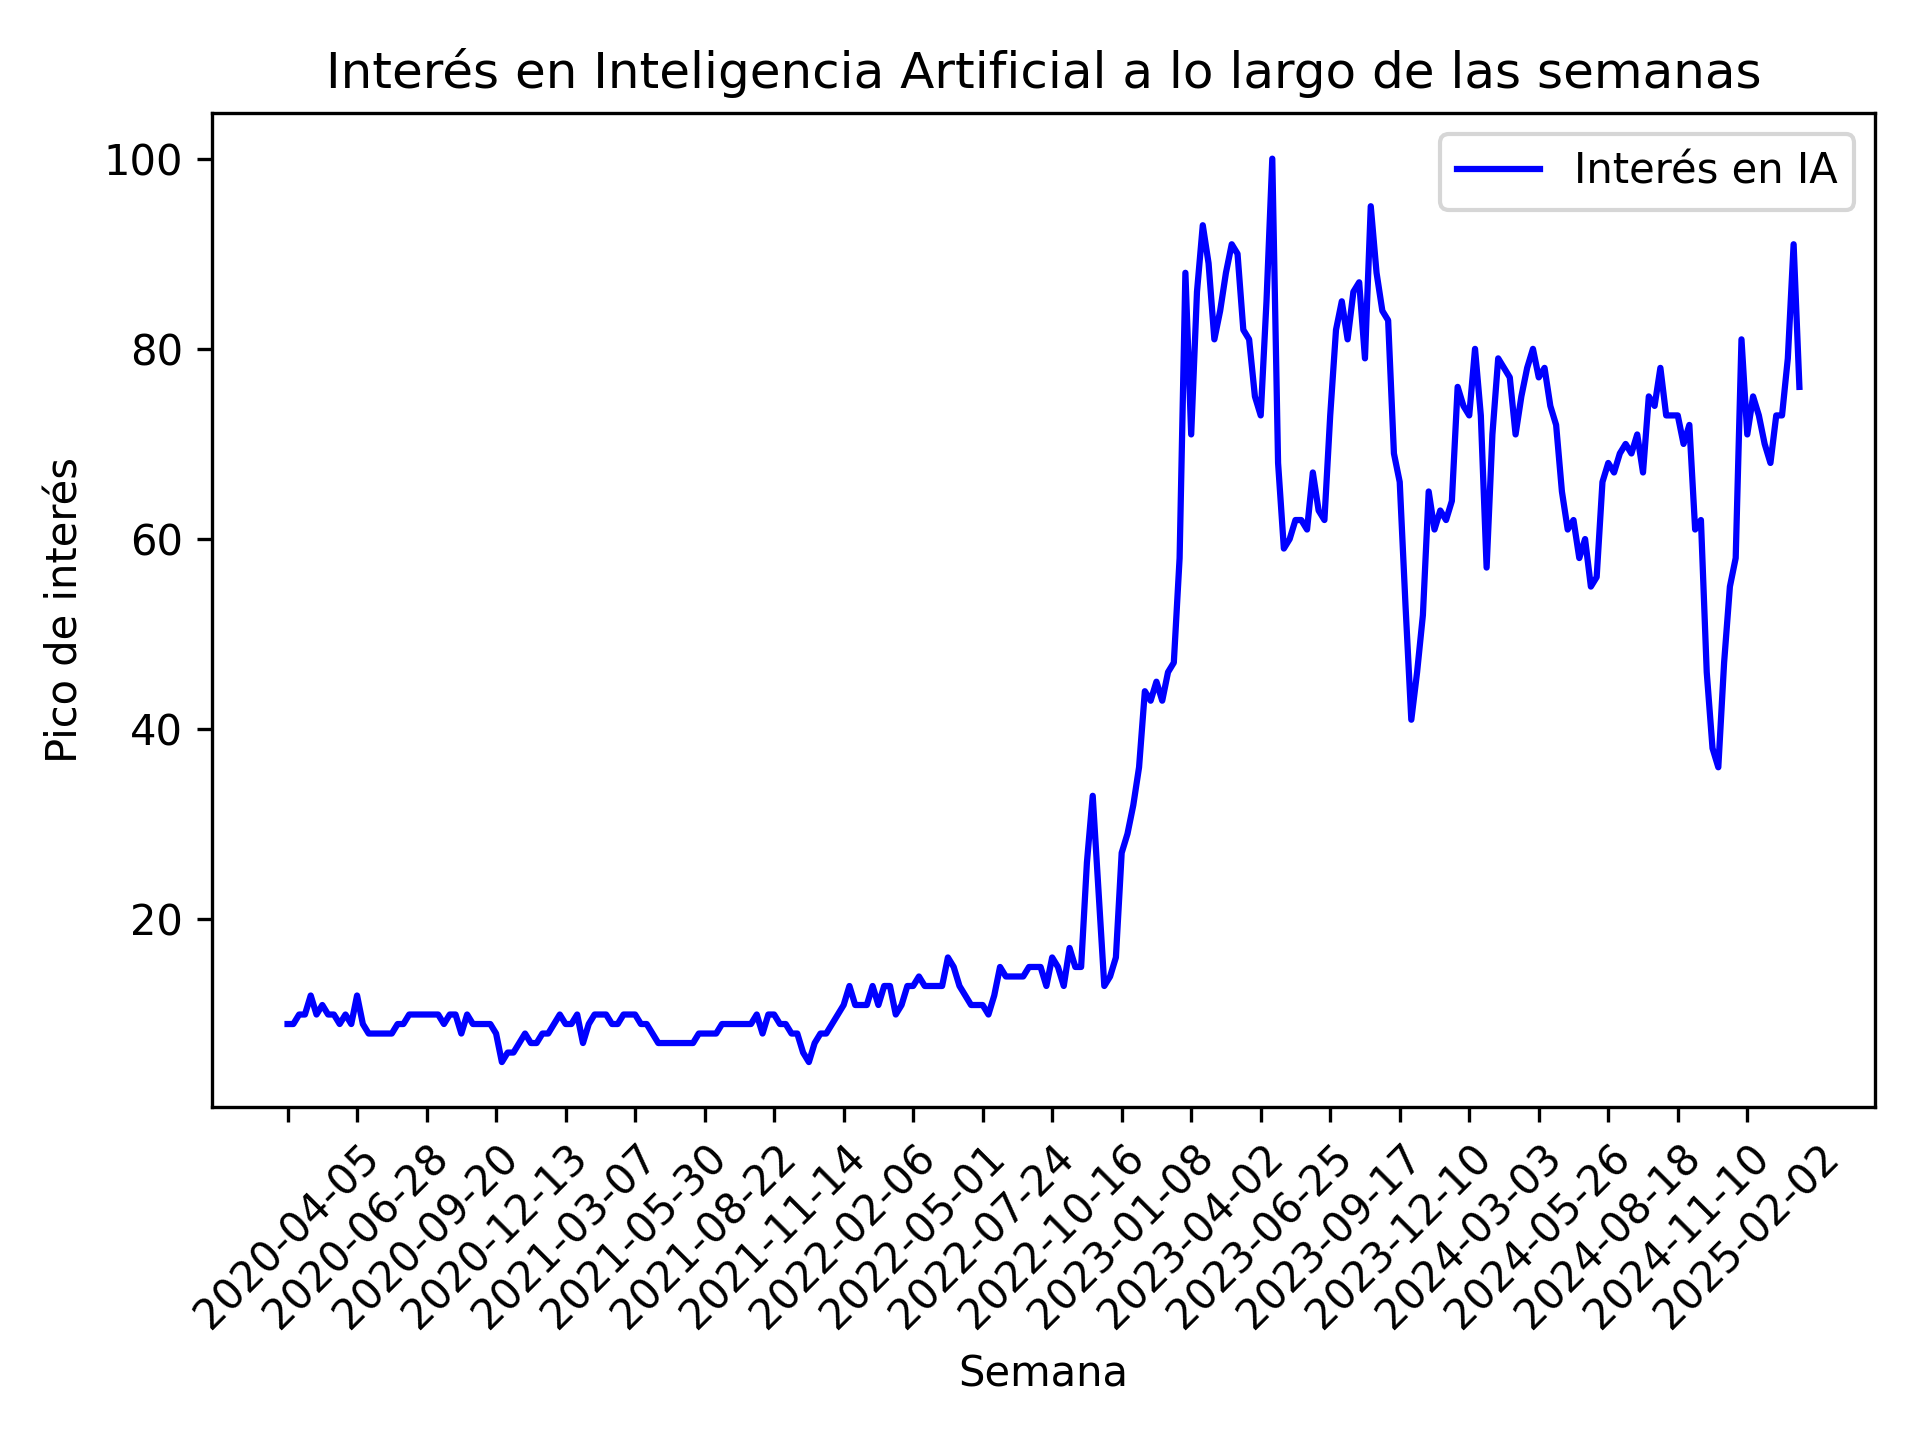
\includegraphics[width=0.7\textwidth]{excels/introduccion/interes_en_ia.png}
   \caption{Evolución del interés público en inteligencia artificial según datos de Google Trends (2020-2025)}
\label{fig:interes_en_inteligencia_artificial}
\end{figure}

El progreso en visión por computador ha sido posible gracias a los avances en redes neuronales convolucionales, que han revolucionado la capacidad de los sistemas para detectar y clasificar objetos en imágenes y vídeos con una gran precisión y velocidad.

Estos algoritmos de visión artificial requieren una potencia computacional significativa tanto para su entrenamiento como para su ejecución. Las CPUs (Unidades Centrales de Procesamiento) tradicionales resultan insuficientes para estas tareas, por lo que la industria ha desarrollado arquitecturas específicas como las GPUs (Unidades de Procesamiento Gráfico), TPUs (Unidades de Procesamiento Tensorial) y DLAs (Aceleradores de Aprendizaje Profundo). Estos componentes están optimizados para ejecutar operaciones de entrenamiento e inferencia de manera eficiente, permitiendo implementar sistemas de visión artificial capaces de procesar información visual en tiempo real. Sin embargo, estos aceleradores suelen presentar un consumo energético elevado, lo que plantea importantes retos de eficiencia y sostenibilidad.


\begin{figure}[H]
   \centering
   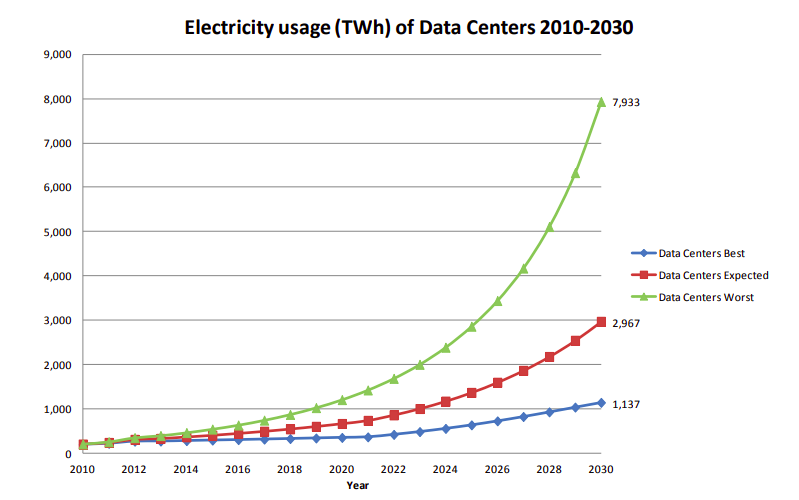
\includegraphics[width=0.7\textwidth]{images/introduccion/consumo_electrico_datacenters.png}
   \caption{Proyección del consumo eléctrico de los centros de datos en el mundo}
\label{fig:consumo_electrico_datacenters}
\end{figure}

Como se observa en la Figura~\ref{fig:consumo_electrico_datacenters}, el consumo eléctrico de los centros de datos en el mundo ha ido aumentando de forma exponencial, lo que plantea un desafío significativo para la sostenibilidad del crecimiento tecnológico \cite{challe6010117}. En el peor escenario, esta tendencia podría llevar a un incremento insostenible en la huella de carbono del sector tecnológico, mientras que en el mejor de los casos, la adopción de tecnologías eficientes podría moderar el crecimiento. Este aumento del consumo energético no solo afecta a los centros de datos, sino también a los dispositivos embebidos y móviles, donde la eficiencia energética es crucial para prolongar la vida útil de las baterías y reducir el impacto ambiental.

Para enfrentar estos desafíos, se han desarrollado diversas técnicas de optimización y compresión que reducen el tamaño y la complejidad de los modelos neuronales manteniendo su rendimiento. Paralelamente, han surgido arquitecturas hardware específicamente diseñadas para la inferencia de modelos de aprendizaje profundo en entornos con restricciones energéticas. En este contexto, los dispositivos de la serie Jetson de NVIDIA destacan por ofrecer un equilibrio entre alto rendimiento en tareas de inteligencia artificial y un consumo energético contenido, ideal para aplicaciones embebidas de visión artificial.

La combinación de redes neuronales convolucionales y aceleradores hardware ha permitido la creación de sistemas de visión artificial que pueden detectar y clasificar objetos en movimiento, lo que es esencial en aplicaciones como la vigilancia, la conducción autónoma y la robótica.

\section{Motivaci\'on}

Los humamos somos capaces de ver y entender el mundo que nos rodea. Dada una imagen, podemos identificar objetos, reconocer patrones y tomar decisiones basadas en la información visual. Sin embargo, esta capacidad no es innata en las máquinas. La visión por computador es la ciencia que busca dotar a las máquinas de la capacidad de interpretar y comprender imágenes y vídeos, emulando la forma en que los humanos percibimos el entorno. 

Como se mencionó anteriormente, la inteligencia artificial ha revolucionado la forma en que interactuamos con la tecnología. Se ha convertido en una herramienta esencial para aplicar soluciones innovadoras en una amplia gama de campos. En particular, la visión por computador ha demostrado ser un área de gran potencial. También la existencia de dispositivos de bajo consumo, como los de la serie Jetson de NVIDIA, ha permitido llevar la inteligencia artificial a entornos de edge computing (cómputo en el borde), donde se acerca el procesamiento de datos a la fuente de información. Esto reduce la latencia y el consumo energético. Con todo esto, se abre un abanico de posibilidades para la implementación de sistemas de visión artificial en aplicaciones industriales.

Centradánose en el ámbito industrial, la detección y clasificación de objetos en movimiento es crucial para optimizar procesos, mejorar la seguridad y aumentar la eficiencia. En la mayoría de entornos productivos, la detección de defectos se realiza de forma manual, lo que puede ser ineficiente y propenso a errores. La automatización de este proceso mediante sistemas de visión artificial puede reducir costos, aumentar la precisión y mejorar la calidad del producto final.


La motivación de este trabajo radica en la necesidad de desarrollar un sistema de visión artificial capaz de detectar y clasificar objetos en movimiento en un entorno industrial, específicamente en una cinta transportadora.


\section{Objetivos}

El objetivo principal de este trabajo es desarrollar un sistema de visión artificial capaz de detectar y clasificar objetos en movimiento en una cinta transportadora utilizando redes neuronales convolucionales y aceleradores hardware de bajo consumo. Para lograr este objetivo, se plantean los siguientes objetivos específicos:

\begin{itemize}
   \item Realizar un estudio del estado del arte en redes neuronales convolucionales, aceleradores hardware de bajo consumo y técnicas avanzadas de optimización para visión artificial.
   \item Desarrollar un conjunto de datos para el entrenamiento y evaluación del sistema, mediante la captura y etiquetado de imágenes de objetos en movimiento.
   \item Diseñar, entrenar y validar un modelo de red neuronal convolucional optimizado para la detección y clasificación en tiempo real de defectos en objetos en movimiento.
   \item Implementar un sistema completo de visión artificial que integre el modelo entrenado con los aceleradores hardware NVIDIA, enfocado en maximizar la eficiencia y minimizar la latencia.
   \item Analizar los cuellos de botella del sistema, y aplicar técnicas específicas de optimización para mejorar el rendimiento y la eficiencia energética.
   \item Cuantificar de manera exhaustiva el rendimiento del sistema mediante métricas precisas de exactitud (mAP, precisión, recall), latencia (FPS) y consumo energético (W, J/inferencia).
   \item Realizar un análisis comparativo sistemático entre diferentes configuraciones de hardware, software y parámetros de optimización para identificar la combinación que ofrezca el mejor equilibrio entre precisión, velocidad y eficiencia energética.
\end{itemize}

\section{Estructura de la memoria}

????? ????????????? ????????????? ????????????? ????????????? ????????????? 

%\section{Notes bibliografiques} %%%%% Opcional

%????? ????????????? ????????????? ????????????? ????????????? ?????????????

%%%%%%%%%%%%%%%%%%%%%%%%%%%%%%%%%%%%%%%%%%%%%%%%%%%%%%%%%%%%%%%%%%%%%%%%%%%%%%%
%                         CAPITOLS (tants com calga)                          %
%%%%%%%%%%%%%%%%%%%%%%%%%%%%%%%%%%%%%%%%%%%%%%%%%%%%%%%%%%%%%%%%%%%%%%%%%%%%%%%

\chapter{Conceptos Previos}

En este capítulo se explicará los conceptos previos que constituyen la base teórica y técnica de este trabajo. Primero, se examinarán los fundamentos en Inteligencia Artificial centrándose en las redes neuronales convolucionales, desde sus bases hasta los modelos más recientes en detección de objetos. A continuación, se analizarán los aceleradores hardware de bajo consumo, con especial énfasis en la arquitectura y capacidades de los dispositivos NVIDIA Jetson. Posteriormente, se estudiarán los algoritmos de seguimiento de objetos en tiempo real, fundamentales para aplicaciones con elementos en movimiento. Finalmente, se explorará la técnica de Slicing Aided Hyper Inference (SAHI), una metodología avanzada para mejorar la detección de objetos pequeños o densamente agrupados. Este marco teórico permitirá contextualizar adecuadamente la solución propuesta para la detección de defectos en objetos en movimiento.

\section{Fundamentos y avances en redes neuronales para visión artificial}
En esta sección se realizará un estudio de las redes neuronales profundas hasta las redes neuronales convolucionales, desde sus fundamentos hasta los modelos más recientes en detección de objetos. Se explicarán los conceptos básicos de las redes neuronales y la evolución de las arquitecturas.

\subsection{Fundamentos de la inteligencia artificial}
La \textit{\textbf{Inteligencia Artificial}} es un campo de estudio que busca desarrollar sistemas capaces de realizar tareas que normalmente requieren inteligencia humana, como el reconocimiento de voz, la toma de decisiones y la comprensión del lenguaje natural. Dentro de este campo, existen diversas subdisciplinas, entre las cuales destacan el \textit{\textbf{Machine Learning}} y el \textit{\textbf{Deep Learning}}.

El \textit{\textbf{Machine Learning}} o aprendizaje automático es una rama de la inteligencia artificial que se centra en el desarrollo de algoritmos y modelos que permiten a las máquinas aprender de los datos y realizar predicciones o tomar decisiones sin ser programadas explícitamente. Este enfoque se basa en la idea de que las máquinas pueden identificar patrones y relaciones en grandes conjuntos de datos, lo que les permite generalizar y adaptarse a nuevas situaciones.

El \textit{\textbf{Deep Learning}} o aprendizaje profundo es una rama del aprendizaje automático que utiliza redes neuronales artificiales con múltiples capas para modelar y resolver problemas complejos. Este enfoque permite aprender representaciones jerárquicas de los datos, donde cada capa extrae características cada vez más abstractas. Una de las arquitecturas fundamentales es el \textit{Multilayer Perceptron} (MLP) o perceptrón multicapa, que consiste en una red de neuronas artificiales organizadas en al menos tres capas: una de entrada, una o más capas ocultas y una capa de salida, como se muestra en la Figura~\ref{fig:multilayer_perceptron} \cite{khan2018guide}. En un MLP, cada neurona recibe un conjunto de entradas ponderadas por pesos, aplica una función de activación no lineal a la suma de estas entradas ponderadas, y produce una salida que se transmite a la siguiente capa. Esta estructura permite al Deep Learning abordar tareas complejas en visión por computador, procesamiento del lenguaje natural y otros dominios con un alto grado de precisión.


\begin{figure}[H]
   \centering
   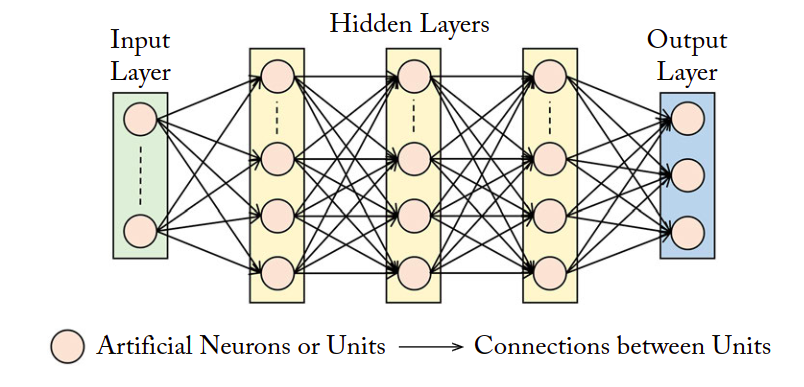
\includegraphics[width=0.6\textwidth]{images/estado_del_arte/multilayer_perceptron.png}
   \caption{Estructura de un perceptrón multicapa (MLP).}
   \label{fig:multilayer_perceptron}
\end{figure}

\subsection{Tareas fundamentales en visión por computador}

La visión por computador aborda el desafío de permitir que las máquinas interpreten y comprendan el contenido visual de imágenes y vídeos. Antes del auge del aprendizaje profundo, se empleaban descriptores de características diseñados manualmente, como el Histograma de Gradientes Orientados (HOG). HOG captura la forma local de los objetos analizando la distribución de las orientaciones de los gradientes en pequeñas regiones de la imagen (celdas y bloques). La Figura~\ref{fig:hog} muestra una visualización de las características HOG extraídas. Aunque útiles en su momento, estos algoritmos "hechos a mano" presentan limitaciones significativas. En particular, no facilitan el aprendizaje por transferencia, es decir, la reutilización de conocimiento aprendido en tareas previas. Además, la complejidad de estas características está intrínsecamente limitada por la capacidad humana para diseñarlas explícitamente. Estos inconvenientes son superados por los algoritmos de aprendizaje automático de características, como las CNN, que aprenden representaciones relevantes directamente de los datos. Por ello, las CNN han demostrado ser más efectivas en tareas complejas, logrando avances significativos en precisión y eficiencia al aprender automáticamente características a partir de grandes conjuntos de datos.

\begin{figure}[H]
   \centering
   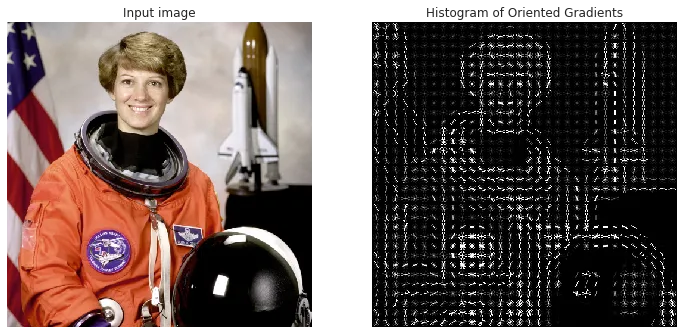
\includegraphics[width=0.6\textwidth]{images/estado_del_arte/HOG_example.png}
   \caption{Ejemplo de HOG aplicado a una imagen.}
   \label{fig:hog}
\end{figure}


En el ámbito del procesamiento de imágenes mediante técnicas de deep learning, existen diversas tareas con diferentes niveles de complejidad:

\begin{enumerate}
    \item \textbf{Clasificación de imágenes}: Es la tarea más básica, donde la red neuronal asigna una etiqueta a toda la imagen. Por ejemplo, determinar si una imagen contiene un perro, gato o coche. El modelo genera un vector de probabilidades para cada clase posible.
    
    \item \textbf{Clasificación con localización}: Además de clasificar el objeto principal, la red también proporciona un cuadro delimitador (bounding box) que indica dónde se encuentra ese objeto en la imagen. Es útil cuando existe un único objeto de interés.
    
   \item \textbf{Detección de objetos}: Extiende la tarea anterior para identificar y localizar múltiples objetos en una imagen. Los algoritmos de detección se dividen principalmente en:
      \begin{itemize}
         \item \textit{Detectores de dos etapas}: Como R-CNN, Fast R-CNN y Faster R-CNN, primero generan propuestas de regiones que podrían contener objetos, y luego clasifican estas regiones. Son más precisos pero computacionalmente más costosos.
         \item \textit{Detectores de una etapa}: Como YOLO (You Only Look Once) y SSD (Single Shot MultiBox Detector), que predicen las cajas delimitadoras y las clases directamente en una sola pasada. Son más rápidos aunque tradicionalmente menos precisos.
      \end{itemize}
      Ambos enfoques proporcionan para cada objeto detectado su clasificación y cuadro delimitador.
    
    \item \textbf{Segmentación}: Es la tarea más compleja, donde la red no solo identifica y localiza objetos, sino que también asigna una etiqueta a cada píxel de la imagen. Esto permite distinguir entre diferentes objetos y sus contornos, facilitando una comprensión más detallada de la escena.
\end{enumerate}

La Figura~\ref{fig:tareas_vision_por_computador} ilustra estas tareas fundamentales en visión por computador. Para este trabajo, nos centraremos en la tarea de detección de objetos, que es esencial para identificar y clasificar varios objetos en movimiento en un vídeo o imagen. 

\begin{figure}[H]
   \centering
   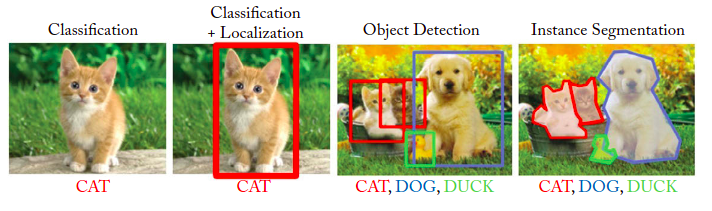
\includegraphics[width=0.8\textwidth]{images/estado_del_arte/diferentes_formas_de_detectar.png}
   \caption{Tareas fundamentales en visión por computador.}
   \label{fig:tareas_vision_por_computador}
\end{figure}

\subsection{Arquitectura y funcionamiento de las CNN}
Las \textit{\textbf{Convolutional Neural Networks}} (CNN) o redes neuronales convolucionales son un tipo específico de red neuronal profunda. Estas redes están diseñadas para procesar imágenes y extraer características relevantes de manera eficiente, lo que las hace especialmente adecuadas para tareas de visión por computador.

\begin{figure}[H]
   \centering
   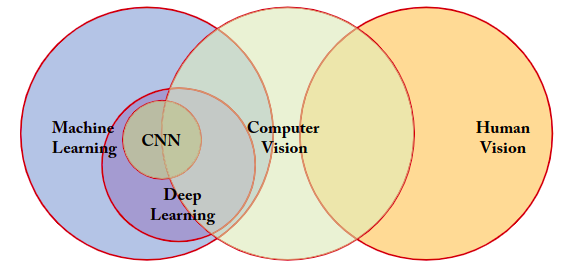
\includegraphics[width=0.6\textwidth]{images/estado_del_arte/diagrama_de_Venn_inteligencia_artificial.png}
   \caption{Relación entre Machine Learning, Deep Learning, CNN, Computer Vision y Human Vision.}
   \label{fig:diagrama_de_Venn_inteligencia_artificial}
\end{figure}

La Figura~\ref{fig:diagrama_de_Venn_inteligencia_artificial} ilustra la relación entre estos conceptos \cite{khan2018guide}. Las CNN son una subcategoría del Deep Learning, que a su vez es una subcategoría del Machine Learning. Además, las CNN están estrechamente relacionadas con la visión por computador, que busca emular la capacidad de los humanos para interpretar imágenes y vídeos.

Las CNN se inspiran en la forma en que los humanos percibimos el mundo visual. Al igual que nuestro sistema visual, que procesa la información de manera jerárquica, las CNN utilizan capas convolucionales para extraer características de bajo nivel (como bordes y texturas) y capas más profundas para identificar patrones y objetos más complejos. Esta jerarquía de características permite a las CNN aprender representaciones ricas y abstractas de los datos visuales.

Estas redes se componen de varias capas, cada una de las cuales realiza operaciones específicas en los datos de entrada. Las capas más comunes y técnicas asociadas en una CNN, que se describen a continuación, son las capas convolucionales, las capas de activación, las capas de pooling, la normalización por lotes y las capas completamente conectadas

Las \textbf{capas convolucionales} utilizan la operación de convolución para extraer características. Esta operación es fundamental en las CNN y consiste en aplicar un filtro (o kernel) a una imagen para extraer características locales. El filtro se desliza sobre la imagen, multiplicando sus valores por los valores de la imagen en cada posición y sumando los resultados. Este proceso genera un mapa de activación que resalta las características relevantes de la imagen.  

\begin{figure}[H]
   \centering
   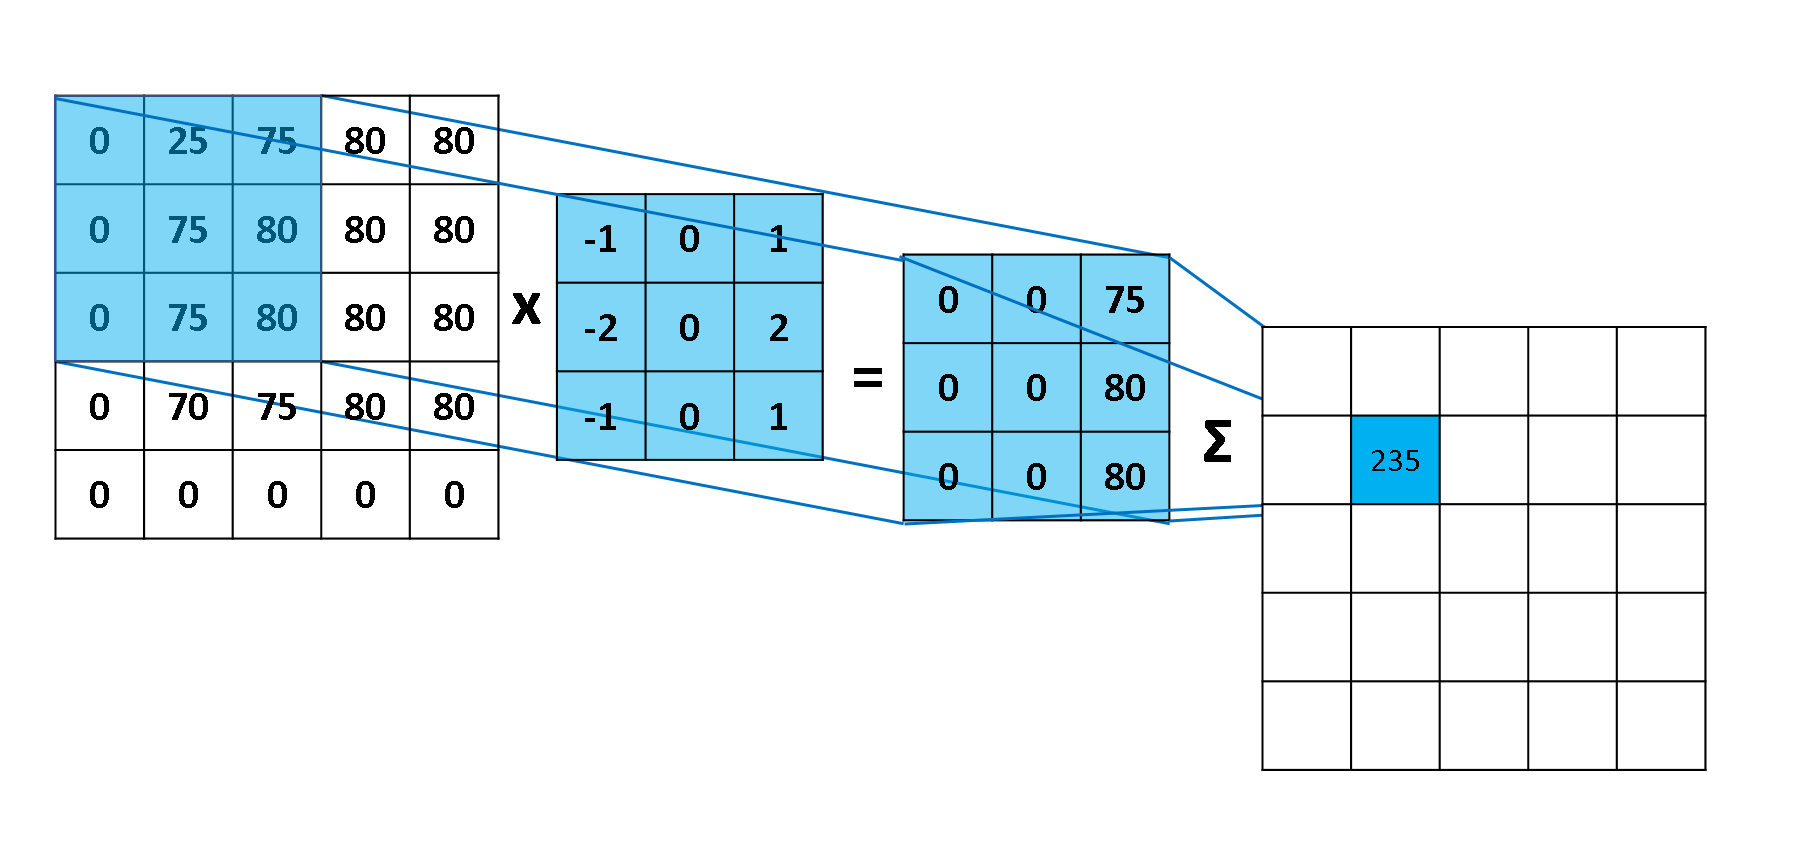
\includegraphics[width=0.7\textwidth]{images/estado_del_arte/operacion_convolucion.png}
   \caption{Operación de convolución sobre los pixeles de una imagen.}
   \label{fig:operacion_convolucion}
\end{figure}

La Figura~\ref{fig:operacion_convolucion}\cite{khan2018guide} ilustra la operación de una capa de convolución. En este ejemplo, se aplica un filtro de $2 \times 2$ (mostrado en verde) a un mapa de características de entrada de $6 \times 6$ (incluyendo un relleno de ceros de 1) con un paso (stride) de 2. El filtro se desliza sobre la entrada, y en cada paso, se realiza una multiplicación elemento a elemento entre el filtro y la región correspondiente de la entrada. La suma de estos productos genera un valor en el mapa de características de salida (mostrado en azul).

\begin{figure}[H]
   \centering
   \begin{subfigure}[b]{0.25\textwidth}
      \centering
      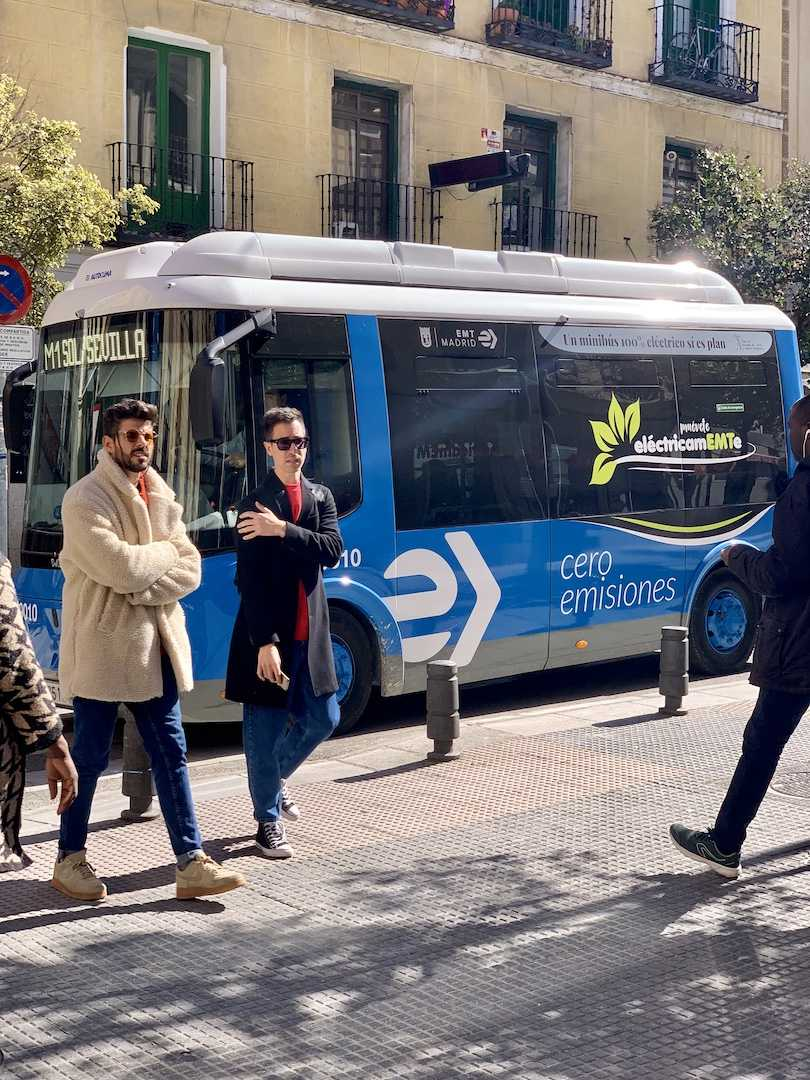
\includegraphics[width=\textwidth]{images/estado_del_arte/bus_original.jpg}
      \caption{Imagen de un autobús.}
      \label{fig:bus_original}
   \end{subfigure}
   \hfill
   \begin{subfigure}[b]{0.7\textwidth}
      \centering
      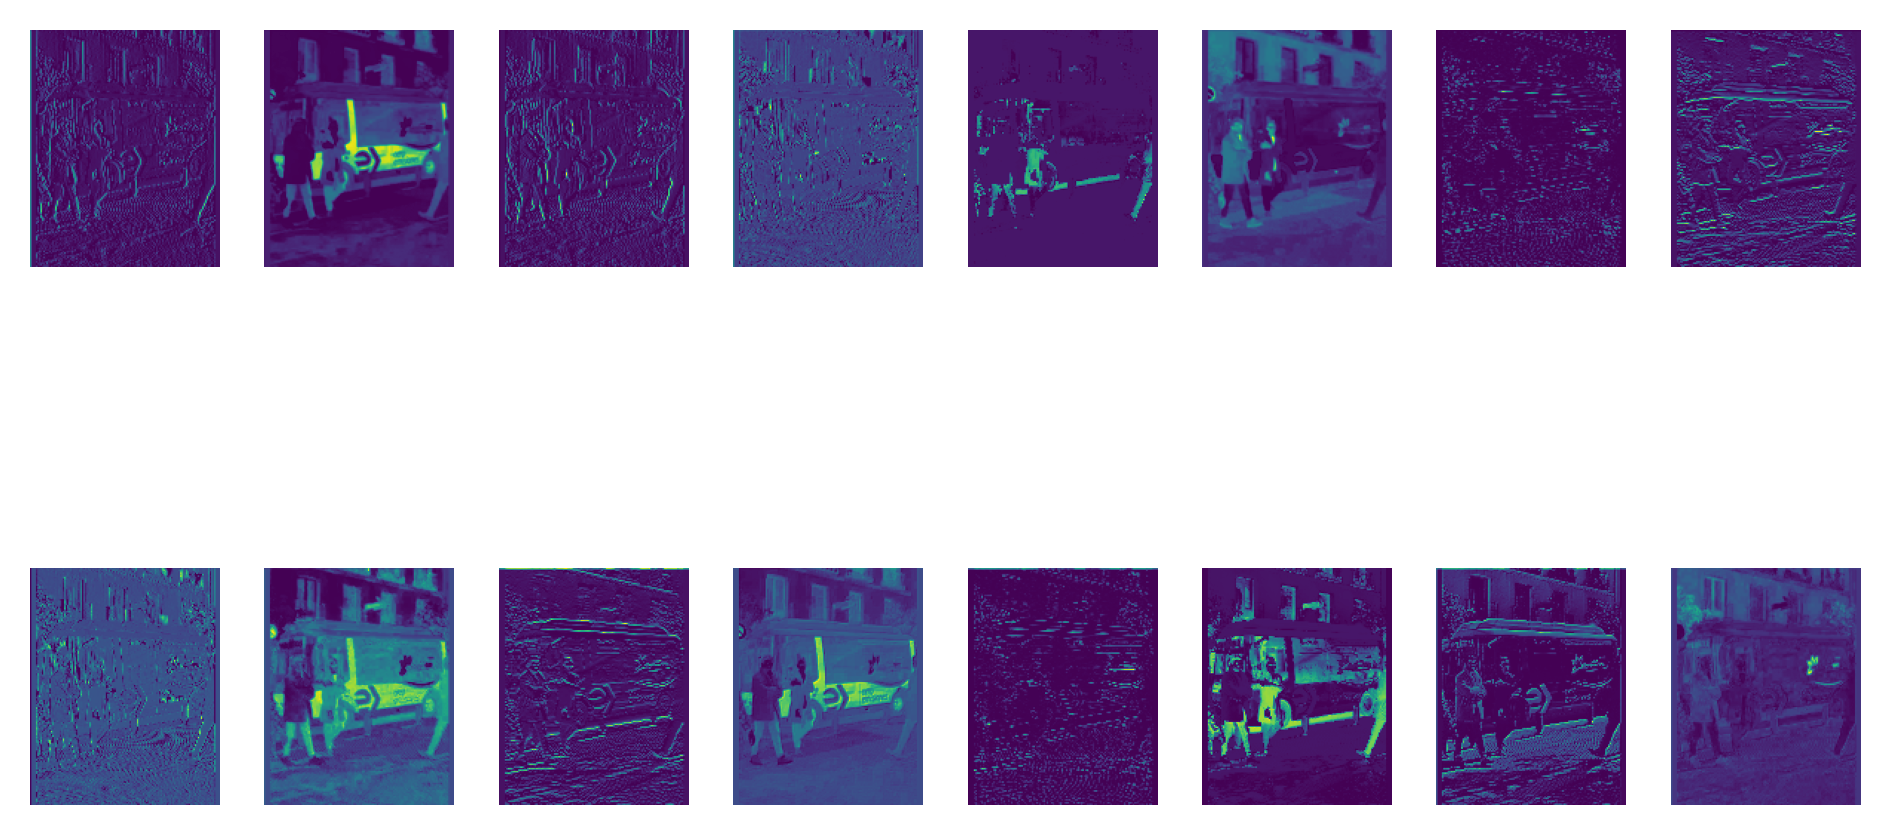
\includegraphics[width=\textwidth]{images/estado_del_arte/bus_primera_capa_convolucion.png}
      \caption{Resultado de la operación de convolución.}
      \label{fig:bus_primera_capa_convolucion}
   \end{subfigure}
   \caption{Proceso de convolución aplicado a una imagen de un autobús.}
   \label{fig:bus_convolucion}
\end{figure}

La Figura~\ref{fig:bus_convolucion} ilustra el proceso de la primera convolución del modelo YOLO11n \cite{yolo11_ultralytics}. En la parte izquierda se muestra la imagen original de un autobús, mientras que en la parte derecha se presenta el resultado de aplicar la operación de convolución. En este caso, los 16 filtros de la primera capa convolucional han detectado diferentes características de la imagen, como bordes y texturas. Este proceso se repite en múltiples capas, lo que permite a la red aprender representaciones cada vez más complejas de la imagen.

Las \textbf{capas de activación}, especialmente la ReLU (Rectified Linear Unit), son fundamentales para introducir no-linealidad en el modelo. La función ReLU transforma cada valor negativo en cero mientras mantiene los valores positivos sin cambios, lo que ayuda a mitigar el problema del desvanecimiento del gradiente y acelera el proceso de entrenamiento. La función ReLU se define como:
\begin{equation}
   f(x) = \begin{cases}
      0 & \text{si } x < 0 \\
      x & \text{si } x \geq 0
   \end{cases}
\end{equation}
Estas capas se aplican típicamente después de cada capa convolucional y completamente conectada.

Las CNN incorporan \textbf{capas de pooling} (o submuestreo). Estas capas desempeñan un papel crucial en la reducción progresiva de la dimensión espacial (ancho y alto) de los mapas de características, lo que conlleva varios beneficios importantes: disminuyen la cantidad de parámetros y la carga computacional, ayudan a controlar el sobreajuste (\textit{overfitting}) al reducir la complejidad del modelo, y proporcionan un cierto grado de invarianza a pequeñas traslaciones y distorsiones. El funcionamiento del pooling implica deslizar una ventana sobre el mapa de características de entrada y aplicar una operación de agregación. Las operaciones más comunes son Max-Pooling, que selecciona el valor máximo dentro de la ventana (eficaz para capturar las características más prominentes, como se ilustra en la Figura~\ref{fig:pooling}), y Average-Pooling, que calcula el valor promedio (tiende a suavizar las características). El resultado es un mapa de características de menor tamaño pero que conserva la información esencial.

\begin{figure}[H]
   \centering
   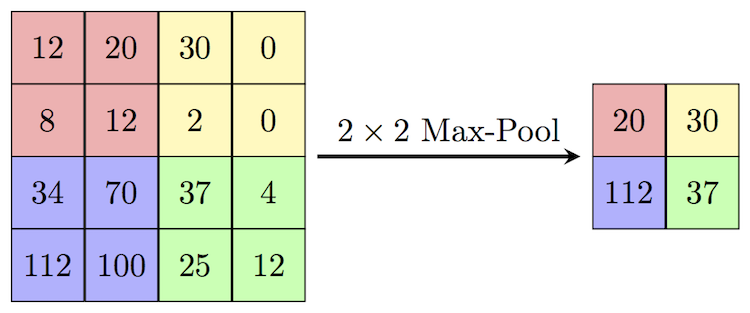
\includegraphics[width=0.6\textwidth]{images/estado_del_arte/max_pooling.png}
   \caption{Ejemplo de operación de max-pooling con una ventana de $2 \times 2$ y un paso de 2. Se selecciona el valor máximo de cada región de color.}
   \label{fig:pooling}
\end{figure}

La \textbf{Normalización por Lotes} (\textit{Batch Normalization}, BN) es una técnica fundamental para mitigar el problema del \textit{cambio interno de covariables} (\textit{internal covariate shift}), que es la alteración de la distribución de las activaciones intermedias durante el entrenamiento. BN opera a nivel de mini-lotes $\mathcal{B} = \{x_1, \dots, x_m\}$, calculando la media $\mu_{\mathcal{B}}$ y la varianza $\sigma^2_{\mathcal{B}}$:
\begin{align}
   \mu_{\mathcal{B}} &= \frac{1}{m} \sum_{i=1}^{m} x_i \\
   \sigma^2_{\mathcal{B}} &= \frac{1}{m} \sum_{i=1}^{m} (x_i - \mu_{\mathcal{B}})^2
\end{align}
Luego, normaliza cada activación $x_i$:
\begin{equation}
   \hat{x}_i = \frac{x_i - \mu_{\mathcal{B}}}{\sqrt{\sigma^2_{\mathcal{B}} + \epsilon}}
\end{equation}
donde $\epsilon$ es una constante pequeña para estabilidad numérica. Para preservar la capacidad expresiva, BN introduce parámetros aprendibles $\gamma$ (escala) y $\beta$ (desplazamiento) para realizar una transformación afín:
\begin{equation}
   y_i = \gamma \hat{x}_i + \beta
\end{equation}
La salida $y_i$ se propaga a la siguiente operación. BN estabiliza y acelera el entrenamiento, permite tasas de aprendizaje más altas y tiene un efecto regularizador que ayuda a prevenir el sobreajuste. Se inserta típicamente después de capas convolucionales o totalmente conectadas, antes de la activación.

En el final de la red, se utilizan \textbf{capas completamente conectadas} (\textit{fully connected}). Estas capas toman las características de alto nivel extraídas por las capas anteriores y las combinan para realizar la tarea final, como la clasificación de objetos. Cada neurona en una capa completamente conectada está conectada a todas las neuronas de la capa anterior. En la salida final, se utiliza una función de activación como Softmax para convertir las salidas en probabilidades de clase. La función Softmax se define como:

\begin{equation}
   \sigma(z_i) = \frac{e^{z_i}}{\sum_{j=1}^{K} e^{z_j}}
\end{equation}
donde $z = (z_1, \dots, z_K)$ es el vector de salidas de la capa anterior para $K$ clases. La función Softmax transforma este vector en un vector de probabilidades $\sigma(z) = (\sigma(z_1), \dots, \sigma(z_K))$, donde cada componente $\sigma(z_i)$ se calcula como se muestra. El resultado es un vector de tamaño $K$ donde cada elemento está en el rango (0, 1) y la suma de todos los elementos es igual a 1 ($\sum_{j=1}^{K} \sigma(z_j) = 1$). Esto permite interpretar la salida como una distribución de probabilidad sobre las $K$ posibles clases.

En la Figura~\ref{fig:cnn_example}\cite{devbreachCNN} se muestra un ejemplo de una red neuronal convolucional (CNN) simple. Esta red incluye capas convolucionales para la extracción de características, capas de activación para introducir no linealidad, capas de pooling para reducir la dimensionalidad y capas completamente conectadas para realizar la clasificación final. La combinación de estas capas permite a las CNN aprender representaciones jerárquicas y complejas de los datos visuales, lo que las convierte en una herramienta poderosa para tareas de visión por computador.

\begin{figure}[H]
   \centering
   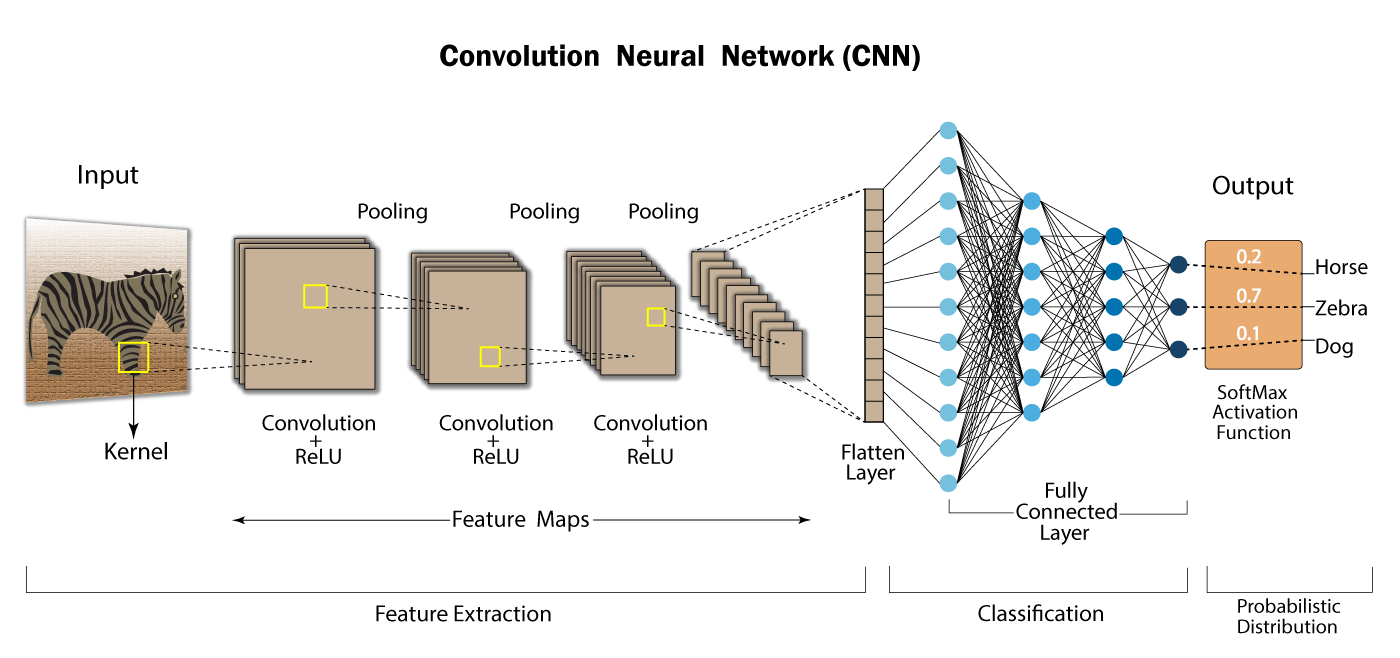
\includegraphics[width=0.9\textwidth]{images/estado_del_arte/cnn_example.png}
   \caption{Ejemplo de una CNN simple.}
   \label{fig:cnn_example}
\end{figure}


Tras comprender la arquitectura interna de las CNN, el siguiente paso es el entrenamiento. Se basa fundamentalmente en el uso de un conjunto de datos etiquetado. Este conjunto contiene una colección de imágenes junto con sus correspondientes etiquetas o anotaciones, que representan la verdad fundamental (\textit{ground truth}). Este conjunto de datos es la base sobre la cual la red aprende a identificar patrones y a realizar predicciones. Durante la fase de entrenamiento, la CNN pasa por un proceso iterativo en el que ajusta sus parámetros internos, específicamente los pesos que conectan sus neuronas y los sesgos aplicados a ellas. Este ajuste es dirigido por un algoritmo de optimización; el Descenso de Gradiente Estocástico (SGD) y sus variantes, como Adam o RMSprop, son opciones comunes para esta tarea. El objetivo principal del algoritmo de optimización es minimizar una función de pérdida predefinida. Esta función de pérdida mide la discrepancia o el error entre las predicciones generadas por la red y las etiquetas reales proporcionadas en los datos de entrenamiento. Típicamente, todo el conjunto de datos de entrenamiento se procesa varias veces en ciclos conocidos como épocas. Este refinamiento iterativo continúa hasta que el rendimiento de la red, evaluado en un conjunto de datos de validación separado (que no se utiliza para el entrenamiento directo), alcanza un nivel satisfactorio. Esto indica que el modelo ha aprendido representaciones significativas y es capaz de generalizar a datos no vistos previamente.

Además, el entrenamiento de las CNN a menudo incorpora técnicas de regularización cruciales, diseñadas para prevenir el sobreajuste (\textit{overfitting}) y mejorar la capacidad del modelo para generalizar a datos nuevos y no vistos. Dos métodos de regularización ampliamente adoptados son el \textit{dropout} y la normalización por lotes (\textit{batch normalization}). El \textit{dropout} funciona desactivando aleatoriamente un cierto porcentaje de neuronas durante cada iteración de entrenamiento. Esto evita que las neuronas individuales se vuelvan excesivamente especializadas o codependientes, obligando a la red a aprender representaciones de características más distribuidas y robustas, que son menos sensibles a la presencia o ausencia de neuronas específicas. 

En escenarios prácticos, desarrollar y entrenar una CNN desde cero puede ser computacionalmente costoso y requerir grandes cantidades de datos etiquetados. Por lo tanto, una estrategia común y muy eficaz consiste en aprovechar modelos preentrenados. Arquitecturas como VGG16, ResNet50 y MobileNetV2, que han sido entrenadas previamente en conjuntos de datos de referencia masivos como ImageNet (que contiene millones de imágenes en miles de categorías) o COCO (centrado en la detección y segmentación de objetos), sirven como puntos de partida potentes. Estos modelos ya han aprendido características jerárquicas ricas a partir de datos visuales diversos. Mediante una técnica conocida como \textit{transfer learning} o aprendizaje por transferencia, estos modelos preentrenados pueden adaptarse eficientemente a tareas nuevas y específicas, incluso con conjuntos de datos personalizados más pequeños. El aprendizaje por transferencia generalmente implica tomar las capas de extracción de características del modelo preentrenado (la base convolucional) y ajustarlas (\textit{fine-tuning}) o añadir nuevas capas de clasificación adaptadas a la tarea objetivo. Este enfoque acelera significativamente el proceso de entrenamiento para la nueva tarea y, a menudo, conduce a un mejor rendimiento en comparación con el entrenamiento desde cero, ya que transfiere eficazmente el conocimiento visual general adquirido durante el entrenamiento inicial a gran escala.





\subsection{Detectores de dos etapas}
Los detectores de dos etapas, funcionan mediante un proceso secuencial: primero generan propuestas de regiones (region proposals) que podrían contener objetos y posteriormente clasifican estas regiones. Este enfoque favorece la precisión, aunque generalmente a costa de un mayor tiempo de procesamiento.

La primera arquitectura exitosa de detección de objetos basada en deep learning fue R-CNN (Regions with CNN features) \cite{girshick2014richfeaturehierarchiesaccurate}. Este modelo introdujo un enfoque de dos etapas que revolucionó el campo. En su primera fase, R-CNN utiliza un algoritmo de búsqueda selectiva (Selective Search) para generar aproximadamente 2,000 propuestas de regiones que podrían contener objetos. Este algoritmo de búsqueda selectiva divide la imágen en nodos y aristas, e iterativamente agrupa estas regiones en función del color, textura, tamaño y forma hasta que se obtienen las propuestas finales. En la figura \ref{fig:selective_search}\cite{explainningAI} se muestra un ejemplo del resultado del algoritmo de búsqueda selectiva.

\begin{figure}[H]
   \centering
   \begin{subfigure}[b]{0.45\textwidth}
      \centering
      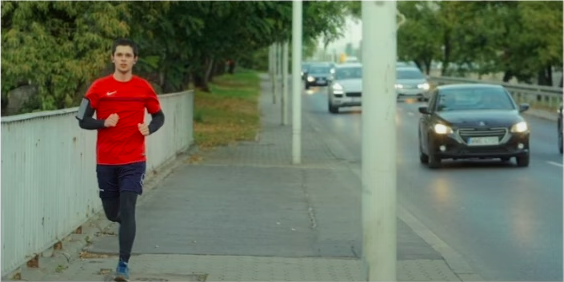
\includegraphics[width=\textwidth]{images/estado_del_arte/selective_search_original.png}
      \caption{Imagen original.}
      \label{fig:selective_search_original}
   \end{subfigure}
   \hfill
   \begin{subfigure}[b]{0.45\textwidth}
      \centering
      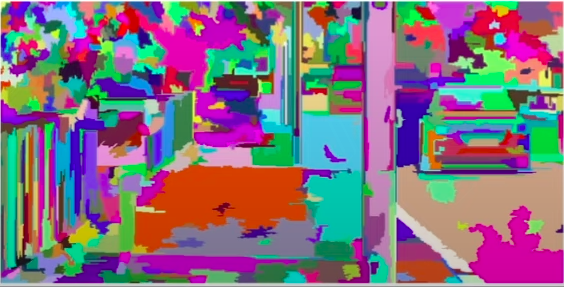
\includegraphics[width=\textwidth]{images/estado_del_arte/selective_search_result.png}
      \caption{Resultado de búsqueda selectiva.}     
      \label{fig:selective_search_result}
   \end{subfigure}
   \caption{Proceso de búsqueda selectiva aplicado a una imagen.}
   \label{fig:selective_search}
\end{figure}

En la segunda fase, cada región propuesta es redimensionada y procesada individualmente por una CNN para extraer características de alto nivel. Estas características alimentan posteriormente a un clasificador SVM (Support Vector Machine) para determinar la categoría del objeto y a un regresor lineal para mejorar la localización del cuadro delimitador. Como se ilustra en la Figura~\ref{fig:r-cnn}, este enfoque fue innovador pero computacionalmente costoso, ya que requiere procesar cada propuesta de región de manera independiente.

\begin{figure}[H]
   \centering
   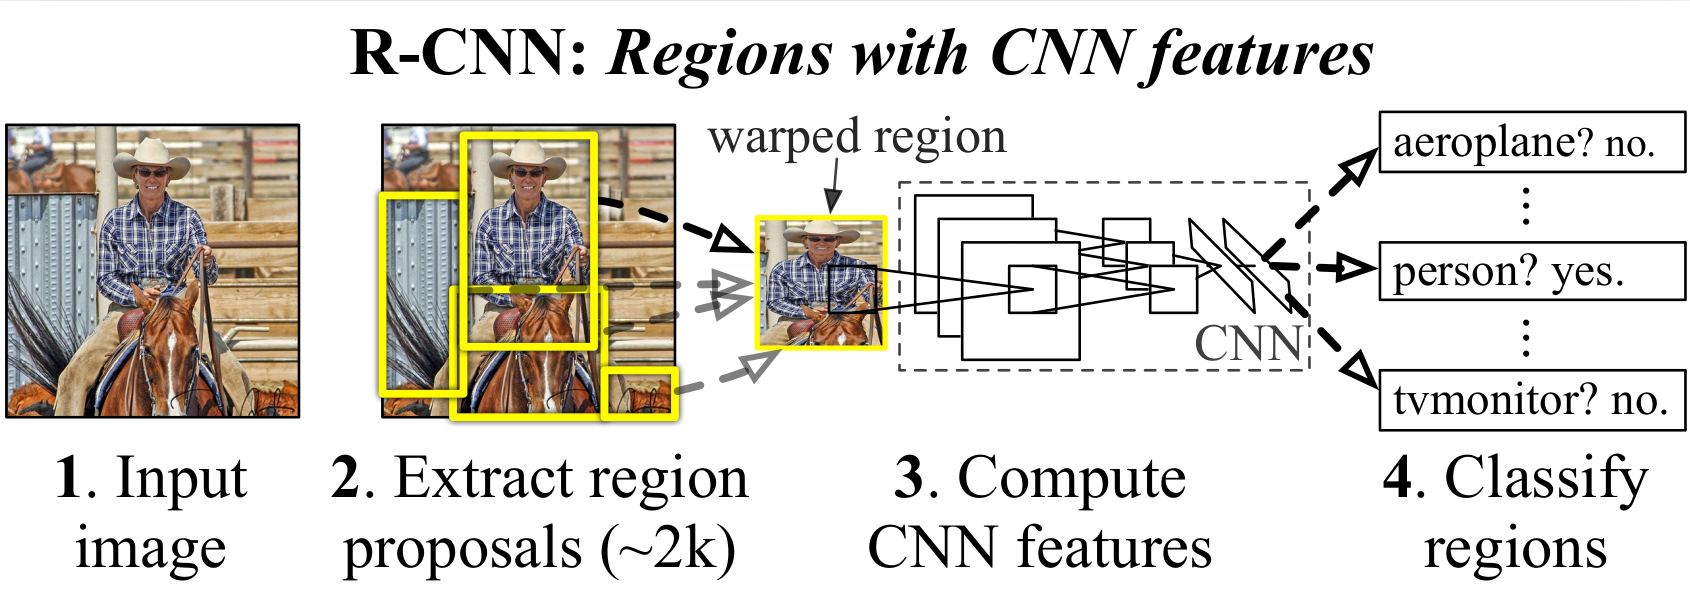
\includegraphics[width=0.6\textwidth]{images/estado_del_arte/R-CNN.png}
   \caption{Arquitectura de R-CNN.}
   \label{fig:r-cnn}
\end{figure}

\subsection{Detectores de una etapa}
%https://www.ultralytics.com/es/glossary/one-stage-object-detectors Explicación de los detectores de 1 etapa por Ultralytics
%https://www.ultralytics.com/glossary/backbone Explicación de la parte de backbone en los detectores de 1 etapa por Ultralytics
%https://www.ultralytics.com/glossary/anchor-free-detectors Explicación de los detectores anchor-free por Ultralytics
%https://sharkyun.medium.com/computer-vision-object-detection-one-stage-vs-two-stage-b05dbff88195 Explicación simple de las diferencias entre los detectores de 2 etapas frente a los de 1 etapa

En contraste con los detectores de dos etapas, los detectores de una etapa (one-stage detectors) adoptan un enfoque más directo y eficiente. Estos detectores realizan la localización y clasificación de objetos simultáneamente en una sola pasada a través de la red, sin necesidad de un paso intermedio de generación de propuestas.

La arquitectura de los detectores de una etapa procesa la imagen completa una única vez, típicamente mediante una red troncal o \textit{backbone} (generalmente una CNN) para la extracción de características. Estas características son posteriormente procesadas por componentes intermedios (\textit{neck}) y alimentadas a una cabeza de detección (\textit{detection head}) que predice simultáneamente las coordenadas de los cuadros delimitadores y las probabilidades de clase. 
Esta arquitectura de una etapa prioriza la velocidad de inferencia, resultando idónea para aplicaciones en tiempo real donde la latencia es un factor crítico, aunque pueda suponer una ligera concesión en la precisión máxima. Modelos representativos de este enfoque incluyen SSD (Single Shot MultiBox Detector)\cite{Liu_2016} y YOLO (You Only Look Once)\cite{redmon2016lookonceunifiedrealtime}. Estos han demostrado un equilibrio eficaz entre rapidez y exactitud, permitiendo la detección en tiempo real incluso en dispositivos con recursos computacionales limitados.

YOLO (You Only Look Once) se destaca como una de las arquitecturas de detección de objetos más populares y efectivas. Concebida específicamente para la detección en tiempo real, YOLO introdujo un enfoque unificado que procesa la imagen completa en una sola pasada, realizando la localización y clasificación de forma simultánea. Esta metodología ha sido fundamental para su adopción en aplicaciones que requieren alta velocidad de procesamiento.

YOLO en su primera versión procesa la imagen completa de una vez. Divide la imagen en una cuadrícula de $S \times S$ celdas. Cada celda es responsable de detectar los objetos cuyo centro se encuentre dentro de ella. Para cada celda, YOLO predice $B$ cuadros delimitadores (bounding boxes) y puntuaciones de confianza para esos cuadros. La puntuación de confianza indica la probabilidad de que haya un objeto en el cuadro y la precisión de la predicción del cuadro. Al mismo tiempo, predice las probabilidades de clase para cada objeto detectado en la celda.

\begin{figure}[H]
   \centering
   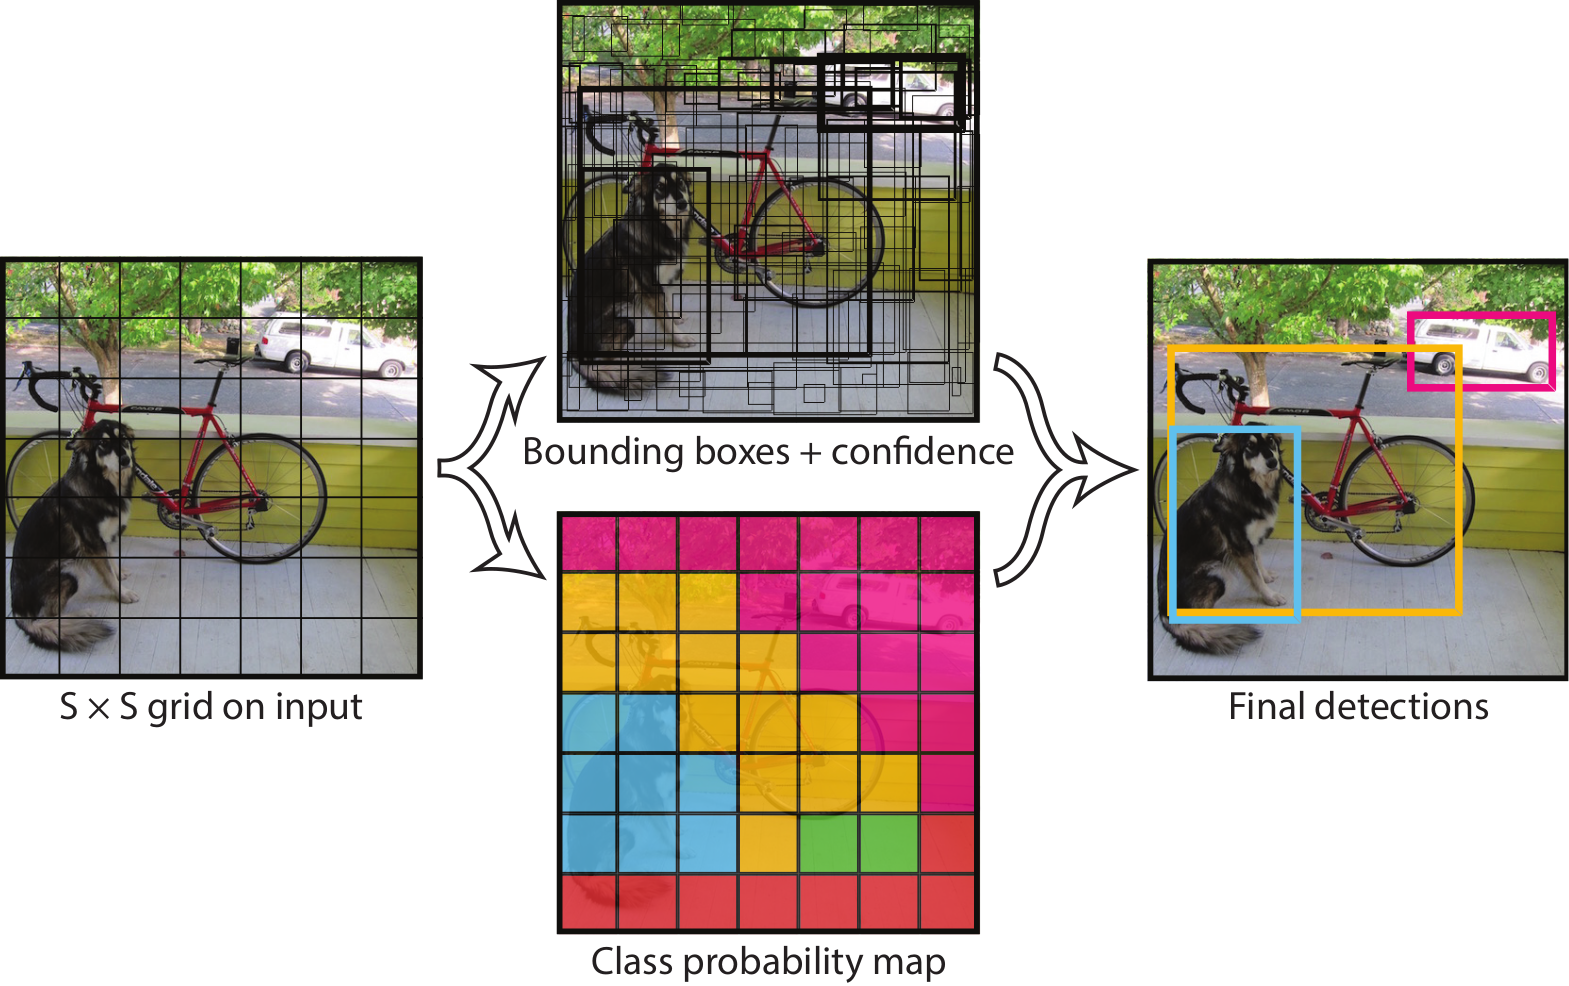
\includegraphics[width=0.8\textwidth]{images/estado_del_arte/yolo_detections_example.png}
   \caption{Ejemplo de detección de objetos utilizando YOLO.}
   \label{fig:yolo_detections_example}
\end{figure}

Como se ilustra en la Figura~\ref{fig:yolo_detections_example}\cite{redmon2016lookonceunifiedrealtime}, YOLO modela la detección como un problema de regresión. Las predicciones del modelo se codifican como una matriz de 3 dimensiones de  $S \times S \times (B * 5 + C)$, donde el factor $5$ corresponde a las coordenadas $x$, $y$, ancho, alto y la puntuación de confianza para cada cuadro delimitador, mientras que $C$ representa el número de clases posibles. Por ejemplo, si se utilizan $B=2$ cuadros delimitadores (por cada celda, es decir, cada celda realiza 2 predicciones) y $C=20$ clases, el tensor de salida tendrá dimensiones $S \times S \times (2 * 5 + 20)$. 

Una vez generadas todas las predicciones, YOLO implementa un post-procesamiento mediante supresión de no máximos (NMS) para eliminar detecciones redundantes y conservar únicamente las más precisas. Este enfoque unificado permite que YOLO procese imágenes a velocidades significativamente mayores que los detectores de dos etapas, mientras mantiene una precisión competitiva, lo que lo hace ideal para aplicaciones en tiempo real como las que se abordan en este trabajo.

\begin{figure}[H]
   \centering
   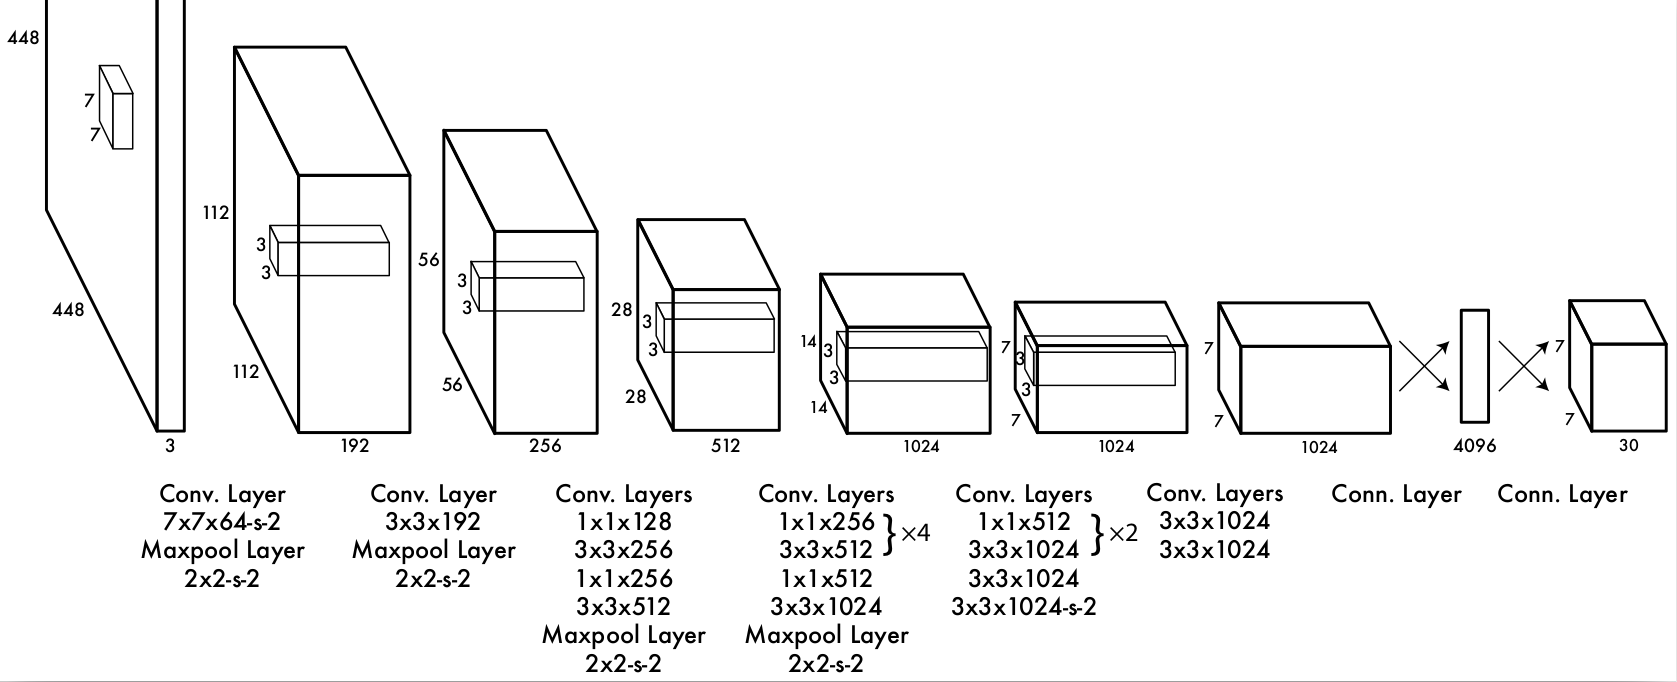
\includegraphics[width=0.8\textwidth]{images/estado_del_arte/yolo_architecture.png}
   \caption{Arquitectura de YOLO}
   \label{fig:yolo_architecture}
\end{figure}

En la Figura~\ref{fig:yolo_architecture} se presenta la arquitectura del modelo primigenio de YOLO \cite{redmon2016lookonceunifiedrealtime}. Esta arquitectura se basa en una red neuronal convolucional que extrae características de la imagen de entrada y las procesa a través de varias capas para generar las predicciones finales. A lo largo de los años, se han desarrollado múltiples versiones y mejoras de YOLO, cada una optimizando aspectos como la precisión, la velocidad y la capacidad de detección de objetos pequeños o densamente agrupados.

En este proyecto, se ha seleccionado YOLO11 \cite{yolo11_ultralytics}, que representa una mejora y optimización sobre las arquitecturas YOLO precedentes. Dicho modelo forma parte de la librería Ultralytics \cite{Jocher_Ultralytics_YOLO_2023}, la cual ofrece una implementación eficaz y sencilla de diversas variantes de YOLO. Las aportaciones de Ultralytics a la comunidad de visión artificial son notables, ya que sus herramientas y recursos agilizan el ciclo de vida (entrenamiento, evaluación, implementación) de los modelos YOLO en múltiples contextos. YOLO11 se ofrece en diversas configuraciones (11n, 11s, 11m, 11l y 11x).
\begin{table}[H]
   \centering
   \resizebox{\textwidth}{!}{%
   \begin{tabular}{l c | cc | c | c}
      \toprule
      Modelo & Tamaño (px) & Latencia CPU ONNX (ms) & Latencia T4 TRT10 (ms) & mAPval (50-95) & Parámetros (M)\\
      \midrule
      YOLO11n & 640 & 56.1 ± 0.8 & 1.5 ± 0.0 & 39.5 & 2.6 \\
      YOLO11s & 640 & 90.0 ± 1.2 & 2.5 ± 0.0 & 47.0 & 9.4 \\
      YOLO11m & 640 & 183.2 ± 2.0 & 4.7 ± 0.1 & 51.5 & 20.1 \\
      YOLO11l & 640 & 238.6 ± 1.4 & 6.2 ± 0.1 & 53.4 & 25.3 \\
      YOLO11x & 640 & 462.8 ± 6.7 & 11.3 ± 0.2 & 54.7 & 56.9 \\
      \bottomrule
   \end{tabular}
   }
   \caption{Análisis comparativo de las variantes de YOLO11 considerando precisión, velocidad y complejidad computacional.}
   \label{tab:yolo11_comparison}
\end{table}

La Tabla \ref{tab:yolo11_comparison} presenta un análisis comparativo de las distintas variantes de YOLO11 evaluadas sobre el dataset COCO \cite{lin2015microsoftcococommonobjects}. Los datos revelan una clara correlación: los modelos más grandes ofrecen mayor precisión (mAP) a costa de mayor complejidad computacional y menor velocidad de procesamiento. Esta escalabilidad permite adaptar la implementación según los requisitos específicos de cada aplicación, balanceando efectivamente el rendimiento con las restricciones computacionales del sistema objetivo.

\subsection{Métricas de evaluación}


Para evaluar el rendimiento de los modelos de detección de objetos, se utilizan métricas específicas que permiten cuantificar la precisión y efectividad del sistema. Entre las métricas más comunes se encuentran:

\begin{itemize}
   \item \textbf{Precisión (Precision)}: Mide la proporción de verdaderos positivos (TP) respecto al total de predicciones positivas realizadas por el modelo. Se calcula como:
   \[
   \text{Precision} = \frac{TP}{TP + FP}
   \]
   donde $FP$ representa los falsos positivos. Una alta precisión indica que el modelo realiza pocas predicciones incorrectas.

   \item \textbf{Recall}: Mide la proporción de verdaderos positivos respecto al total de objetos relevantes en la imagen. Se calcula como:
   \[
   \text{Recall} = \frac{TP}{TP + FN}
   \]
   donde $FN$ representa los falsos negativos. Un alto recall indica que el modelo es capaz de detectar la mayoría de los objetos relevantes, aunque pueda incluir algunas predicciones incorrectas.

   \item \textbf{IoU (Intersection over Union)}: Mide la superposición entre el cuadro delimitador predicho y el cuadro delimitador real. Se calcula como:
   \[
   \text{IoU} = \frac{\text{Area de interseccion}}{\text{Area de union}}
   \]

   Una IoU alta indica que el modelo ha localizado correctamente el objeto. Generalmente, se considera que una IoU superior a 0.5 indica una detección correcta.

   \item \textbf{mAP (mean Average Precision)}: Es una métrica que combina precisión y recall, promediando la precisión a diferentes niveles de recall. Se utiliza para evaluar el rendimiento general del modelo en múltiples clases. 
   
   El cálculo del mAP se realiza en varios pasos: primero, para cada clase se calcula la curva PR (Precision-Recall) y se obtiene el Average Precision (AP), que representa el área bajo esta curva. Luego, el mAP se obtiene como la media de todos los AP de las diferentes clases. En detección de objetos, el mAP suele incorporar diferentes umbrales de IoU (Intersection over Union), expresándose como mAP@IoU=0.5 o mAP@IoU=0.5:0.95. Esta métrica es especialmente útil cuando las clases están desequilibradas, ya que da igual importancia a clases minoritarias y mayoritarias. Un valor de mAP cercano a 1 indica un modelo con alta precisión y recall en todas las clases.

   \item \textbf{Latencia}: Mide el tiempo que tarda el modelo en procesar una imagen y generar una predicción se mide en milisegundos (ms) y un valor bajo indica que el modelo es capaz de realizar inferencias rápidamente.
   
   \item \textbf{FPS (Frames Per Second)}: Mide la velocidad de procesamiento del modelo, indicando cuántas imágenes puede procesar por segundo un alto valor de FPS indica que el modelo es capaz de realizar inferencias rápidamente.
   \item \textbf{F1 Score}: Es la media armónica entre precisión y recall, proporcionando un balance entre ambos. Se utiliza para evaluar el rendimiento del modelo en situaciones donde hay un desbalance entre clases. Se calcula como:
   \[
   \text{F1 Score} = 2 \cdot \frac{\text{Precision} \cdot \text{Recall}}{\text{Precision} + \text{Recall}}
   \]

   Un F1 Score alto indica que el modelo tiene un buen equilibrio entre precisión y recall, lo que es especialmente importante en aplicaciones donde tanto la detección correcta como la minimización de falsos positivos son críticas.

\end{itemize}


\section{Aceleradores de procesamiento gráfico}
Un aspecto fundamental para el despliegue eficiente de modelos de inteligencia artificial es el hardware utilizado para su ejecución. A continuación, se analizan los principales aspectos de los aceleradores de procesamiento gráfico y su importancia en aplicaciones de visión artificial.

\subsection{Limitaciones del hardware tradicional}

La Dennard Scaling, formulada por Robert Dennard en 1974, establecía que a medida que los transistores se reducían de tamaño, su consumo de energía por unidad de área se mantenía constante. Esto significaba que, al reducir el tamaño de los transistores a la mitad, su área se reducía a un cuarto, pero su consumo de energía por unidad de área permanecía igual. Como resultado, el consumo total de energía se reducía a la mitad, permitiendo aumentar la frecuencia de reloj y el número de transistores sin incrementar significativamente el consumo total de energía. Este principio fue fundamental para el avance exponencial en el rendimiento de los procesadores durante décadas. Sin embargo, a partir de 2005, la Dennard Scaling dejó de cumplirse debido a varios factores físicos fundamentales. A escalas nanométricas, los efectos cuánticos y las fugas de corriente se volvieron significativos, impidiendo que el consumo de energía por unidad de área se mantuviera constante.

Por otro lado, la ley de Moore, formulada por Gordon Moore en 1965, predecía que el número de transistores en un chip se duplicaría aproximadamente cada año, predicción que posteriormente se ajustó a cada dos años. Durante décadas, esta ley se cumplió con notable precisión, permitiendo un crecimiento exponencial en la capacidad de procesamiento. Sin embargo, a medida que los transistores se acercan a escalas atómicas (actualmente en torno a los 3-5 nanómetros), los límites físicos y los desafíos de fabricación han ralentizado significativamente este ritmo de avance. Los costes de investigación y desarrollo para mantener esta tendencia se han disparado, y los beneficios en términos de rendimiento por transistor se han reducido.

\begin{figure}[H]
   \centering
   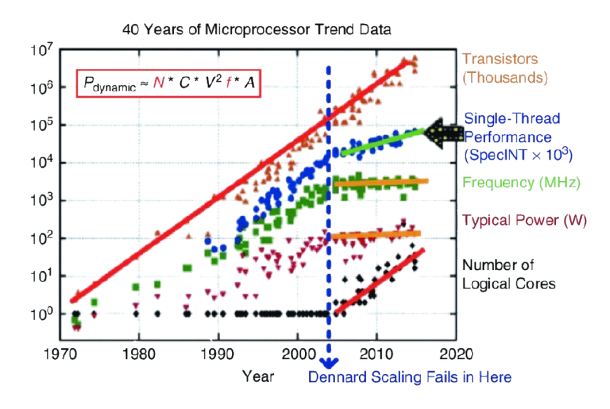
\includegraphics[width=0.8\textwidth]{images/estado_del_arte/dennard_scaling.png}
   \caption{Evolución histórica de las características de los microprocesadores (1970-2020).}
   \label{fig:dennard_scaling}
\end{figure}

En la Figura~\ref{fig:dennard_scaling}\cite{DennardScaling} se ilustra claramente el impacto combinado del fin de la Dennard Scaling y el estancamiento de la ley de Moore. La gráfica muestra cinco métricas fundamentales en escala logarítmica: el número de transistores (triángulos naranja) que sigue la ley de Moore, el rendimiento de un solo hilo (círculos azules), la frecuencia de reloj (cuadrados verdes), el consumo de potencia (triángulos invertidos morados) y el número de núcleos lógicos (rombos negros). La ecuación de potencia dinámica ($P_{dynamic} \approx N * C * V^2 * f * A$) explica la relación entre el número de transistores ($N$), la capacitancia ($C$), el voltaje ($V$), la frecuencia ($f$) y el factor de actividad ($A$).

El punto de inflexión en 2005, marcado como \textit{Dennard Scaling Fails in Here}, marca el momento en que la industria tuvo que cambiar radicalmente su estrategia. La frecuencia de reloj se estancó en torno a los 3-4 GHz, el rendimiento por núcleo comenzó a crecer más lentamente, y como respuesta, se adoptaron dos estrategias principales: el aumento del número de núcleos y la estabilización del consumo de potencia alrededor de los 100W. Este fenómeno ha llevado a la industria a buscar alternativas como las arquitecturas de dominio específico para continuar mejorando el rendimiento de los sistemas computacionales.

\subsection{Arquitectura y funcionamiento de las GPUs}

Las GPUs (Unidades de Procesamiento Gráfico) representan un claro ejemplo de arquitecturas de dominio específico, diseñadas para maximizar el rendimiento en tareas altamente paralelizables. El diseño de las GPUs sigue el paradigma \textit{many-core}, lo que implica la integración de miles de núcleos de procesamiento relativamente simples en un solo chip. Esta arquitectura permite que las GPUs ejecuten múltiples hilos de manera concurrente, lo que resulta especialmente beneficioso para cargas de trabajo que pueden dividirse en tareas independientes.

El modelo de programación de las GPUs está basado en la ejecución masiva de hilos, organizados en bloques y rejillas (\textit{blocks} y \textit{grids}), según la terminología de CUDA, el modelo de programación desarrollado por NVIDIA. Cada hilo ejecuta la misma función, conocida como \textit{kernel}, pero opera sobre diferentes fragmentos de datos. Este enfoque, conocido como SIMT (Single Instruction, Multiple Threads), permite aprovechar al máximo el paralelismo inherente a muchas aplicaciones de inteligencia artificial, como el entrenamiento y la inferencia de redes neuronales.

\begin{figure}[H]
   \centering
   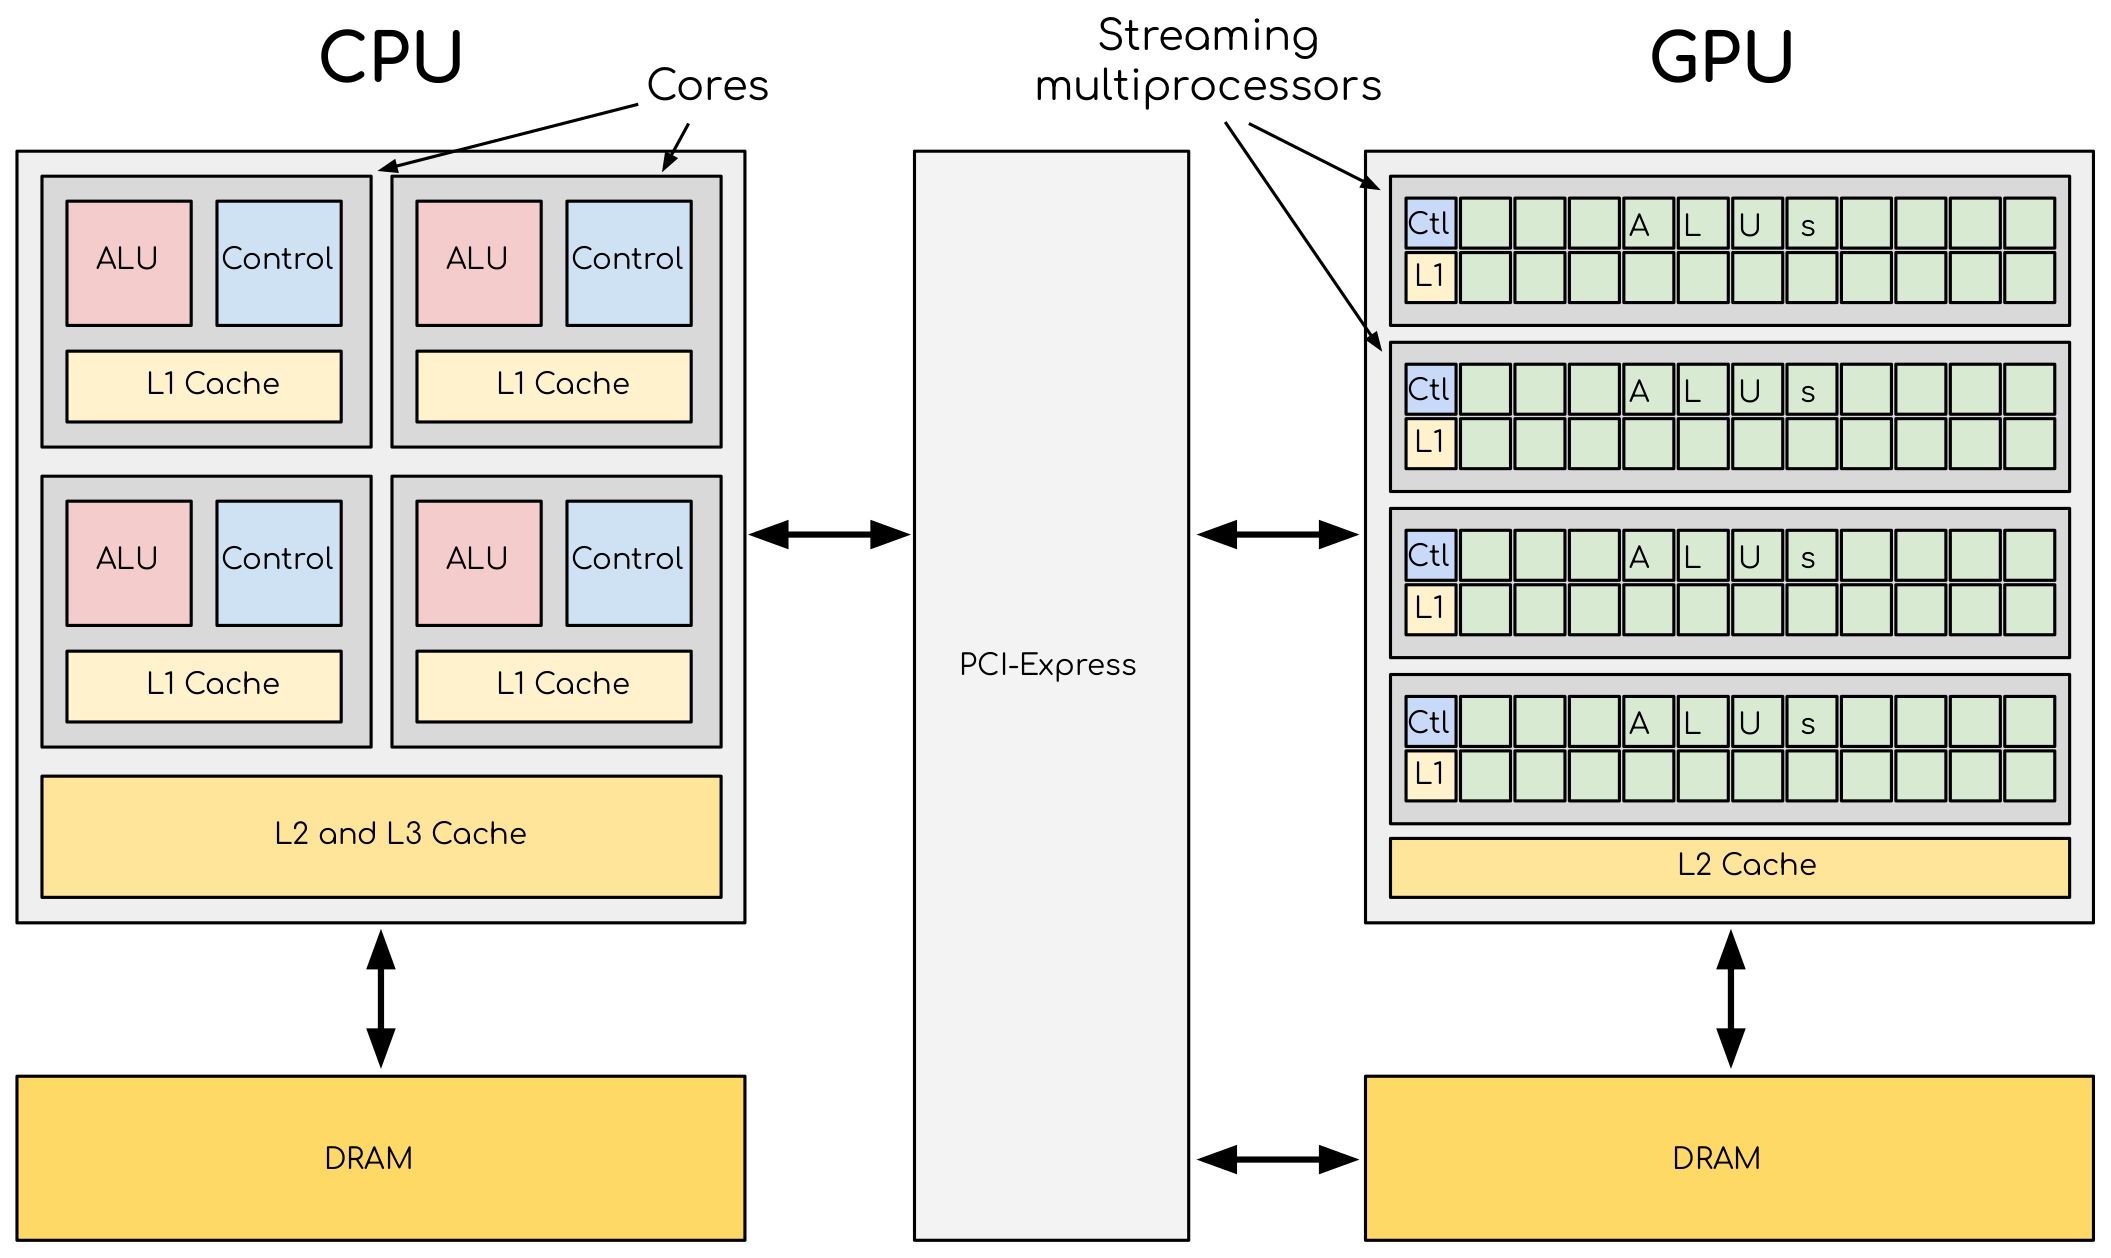
\includegraphics[width=0.8\textwidth]{images/estado_del_arte/cpu_vs_gpu.png}
   \caption{Comparativa de arquitecturas CPU y GPU.}
   \label{fig:cpu_vs_gpu}
\end{figure}
La figura \ref{fig:cpu_vs_gpu}\cite{enccs_gpu_ecosystem} ilustra las diferencias arquitectónicas entre CPU y GPU. Las CPUs constan de un número reducido de núcleos (generalmente entre 4 y 64) optimizados para un alto rendimiento secuencial, donde cada núcleo dispone típicamente de caché y unidad de control privadas. En cambio, las GPUs se basan en una arquitectura \textit{many-core}, integrando miles de núcleos más simples diseñados para el paralelismo masivo, aunque con menor rendimiento individual por núcleo. Estos núcleos de GPU suelen compartir recursos como la caché y las unidades de control, lo que posibilita empaquetar una mayor cantidad de unidades de procesamiento en el mismo chip y, consecuentemente, alcanzar una mayor densidad de cómputo.


NVIDIA ha desempeñado un papel fundamental en el desarrollo de aceleradores para inteligencia artificial, estableciendo un ecosistema robusto que abarca tanto hardware como software. Su enfoque ha permitido optimizar el rendimiento de los modelos de IA, facilitando su implementación en una amplia variedad de aplicaciones.

La programación de GPUs se realiza mediante lenguajes y APIs especializadas como CUDA y OpenCL, que permiten al desarrollador controlar explícitamente la distribución de datos y tareas entre los distintos núcleos. El éxito en este ámbito depende crucialmente de la capacidad para identificar y explotar el paralelismo inherente a los algoritmos, así como de una gestión eficiente de la memoria, dado que el acceso a la memoria global de la GPU es significativamente más lento que el acceso a la memoria compartida entre hilos de un mismo bloque.

NVIDIA ha sido una figura central en la evolución de la aceleración de IA, realizando contribuciones clave que han modelado el campo. Fue pionera en la computación de propósito general en GPUs (GPGPU) con la introducción de CUDA en 2006, una plataforma que permitió utilizar la masiva capacidad de procesamiento paralelo de las GPUs para tareas computacionales generales, extendiendo su uso más allá de los gráficos tradicionales. Complementando esto, NVIDIA ha desarrollado un ecosistema de software robusto y optimizado, que incluye bibliotecas fundamentales como cuDNN, específica para redes neuronales profundas, y cuBLAS, para operaciones de álgebra lineal básica, ambas esenciales para el desarrollo eficiente en inteligencia artificial. En el frente del hardware, la compañía ha impulsado la innovación con el desarrollo de componentes especializados como los Tensor Cores, diseñados específicamente para acelerar las operaciones matriciales intensivas que son comunes en el entrenamiento e inferencia de modelos de IA. Como resultado de estas continuas innovaciones y la creación de un ecosistema integral, NVIDIA ha logrado establecer estándares de facto para el hardware y software utilizados en la aceleración de IA, consolidándose como la plataforma preferida en una amplia gama de entornos, desde grandes centros de datos hasta sistemas embebidos con recursos limitados.


\subsection{Serie Jetson: Dispositivos de IA de bajo consumo}
La serie Jetson de NVIDIA constituye una familia de módulos computacionales diseñados específicamente para habilitar la inteligencia artificial y el aprendizaje profundo en dispositivos de borde (edge devices). Estos sistemas compactos y de bajo consumo son fundamentales para aplicaciones que requieren procesamiento local de datos con alta capacidad de cómputo.

El enfoque principal de la serie Jetson es la computación en el borde (edge computing), un paradigma que acerca el procesamiento de datos y la inteligencia artificial a la fuente donde se generan. Esto resulta crucial en aplicaciones donde la latencia, el ancho de banda limitado o la privacidad son factores críticos, ya que evita la necesidad de enviar grandes volúmenes de datos a la nube para su análisis. Los dispositivos Jetson están optimizados para operar bajo restricciones significativas de energía, tamaño y coste, características típicas de los entornos embebidos y de borde.

Cada módulo Jetson se basa en una arquitectura System-on-Chip (SoC), que integra múltiples componentes de procesamiento en un único circuito integrado. Esto incluye núcleos de CPU basados en la arquitectura ARM, potentes núcleos de GPU NVIDIA con arquitecturas modernas, y en algunos modelos, aceleradores de hardware dedicados como los Deep Learning Accelerators (DLAs). Esta integración permite una alta eficiencia computacional y energética, reduce la huella física del sistema y simplifica el diseño de la placa portadora, resultando en soluciones más compactas y eficientes.

Un pilar fundamental del diseño de la serie Jetson es la optimización de la eficiencia energética. Estos dispositivos están diseñados para ofrecer un alto rendimiento computacional por cada vatio de energía consumido (TOPS/W), esencial para aplicaciones embebidas con fuentes de alimentación limitadas o restricciones térmicas. La capacidad de configurar diferentes perfiles de energía permite ajustar dinámicamente el equilibrio entre rendimiento y consumo.

Más allá del hardware, el valor de la plataforma Jetson reside en su ecosistema de software integral, proporcionado a través del NVIDIA JetPack SDK. Este paquete incluye el sistema operativo Linux optimizado (L4T), controladores, bibliotecas aceleradas por GPU como CUDA, cuDNN y TensorRT, además de herramientas de desarrollo y documentación. Esta plataforma unificada simplifica el ciclo de desarrollo, desde la creación y entrenamiento de modelos hasta su optimización y despliegue en los dispositivos Jetson, acelerando la innovación.

\begin{table}[H]
   \centering
   \resizebox{\textwidth}{!}{%
   \begin{tabular}{l | c | c | c | c | c}
      \toprule
      Modelo & AI Performance & GPU & GPU Max Freq. & CPU & Memoria \\
      \midrule
      Jetson AGX Orin & 275 TOPS & 2048-core Ampere, 64 Tensor Cores & 1.3 GHz & 12-core Cortex-A78AE, 3MB L2 + 6MB L3, 2.2 GHz & 64GB LPDDR5, 204.8GB/s \\
      Jetson Orin Nano & 67 TOPS & 1024-core Ampere, 32 Tensor Cores & 1020 MHz & 6-core Cortex-A78AE, 1.5MB L2 + 4MB L3, 1.7 GHz & 8GB LPDDR5, 102 GB/s \\
      Jetson AGX Xavier & 32 TOPS & 512-core Volta, 64 Tensor Cores & 1377 MHz & 8-core Carmel v8.2, 8MB L2 + 4MB L3, 2.2 GHz & 32GB LPDDR4x, 136.5GB/s \\
      \bottomrule
   \end{tabular}
   }
   \caption{Comparativa técnica entre diferentes modelos NVIDIA Jetson.}
   \label{tab:jetson_comparison}
\end{table}

La tabla \ref{tab:jetson_comparison}\cite{nvidia_jetson_modules} presenta una comparativa técnica entre diferentes modelos de la serie Jetson. Cada modelo está diseñado para satisfacer diferentes necesidades y requisitos de rendimiento, lo que permite a los desarrolladores seleccionar el módulo más adecuado para su aplicación específica. Para este trabajo, se han utilizado los tres modelos de la tabla y se han comparado sus resultados.

\begin{figure}[H]
   \centering
   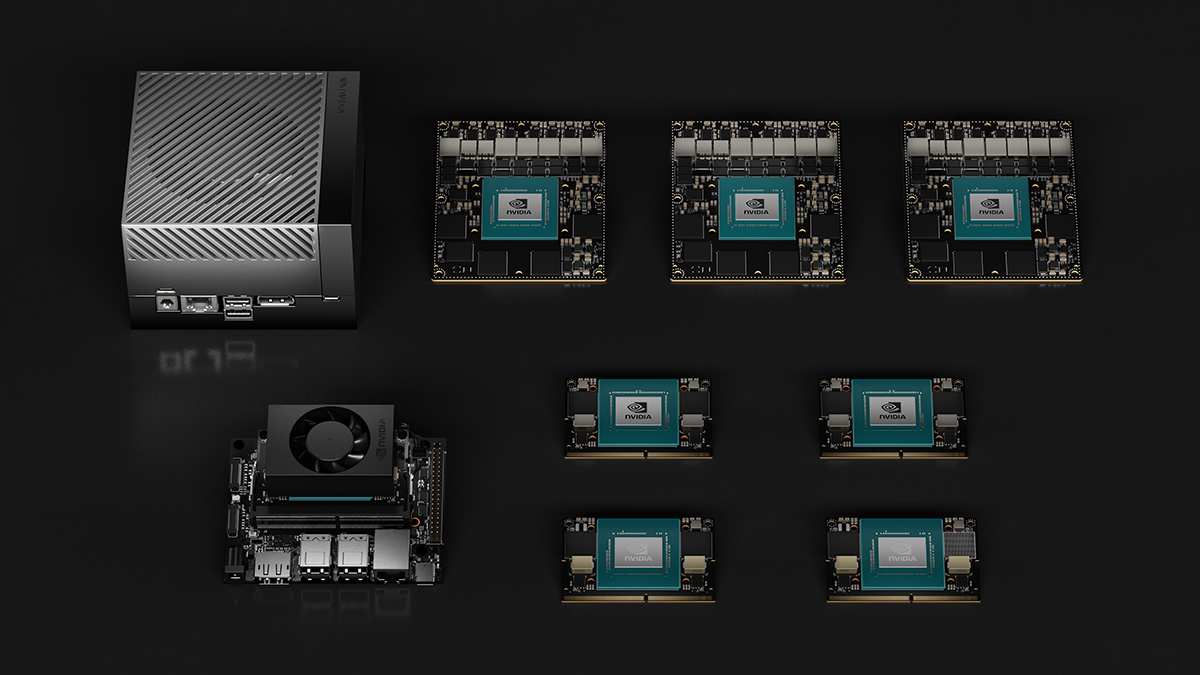
\includegraphics[width=0.8\textwidth]{images/estado_del_arte/jetson_family.png}
   \caption{Módulos Jetson de NVIDIA.}
   \label{fig:jetson_modules}
\end{figure}

\subsection{TensorRT}
NVIDIA TensorRT es un ecosistema diseñado específicamente para optimizar modelos de aprendizaje profundo y lograr una inferencia de alto rendimiento en hardware NVIDIA. Funciona como un compilador y motor de ejecución que transforma modelos entrenados en versiones altamente eficientes para despliegue.

TensorRT aplica optimizaciones avanzadas a nivel de grafo, como la fusión de capas computacionales y la selección de kernels optimizados para la plataforma específica. Además, ofrece un soporte robusto para la cuantización, permitiendo que los modelos operen con precisión numérica reducida (como FP16, FP8, FP4 o enteros) con mínima pérdida de exactitud. Esta reducción de precisión, aplicable tanto post-entrenamiento como mediante entrenamiento consciente de la cuantización, disminuye significativamente la latencia y los requisitos de memoria, lo cual es crucial para aplicaciones en tiempo real y sistemas embebidos.

\begin{figure}[H]
   \centering
   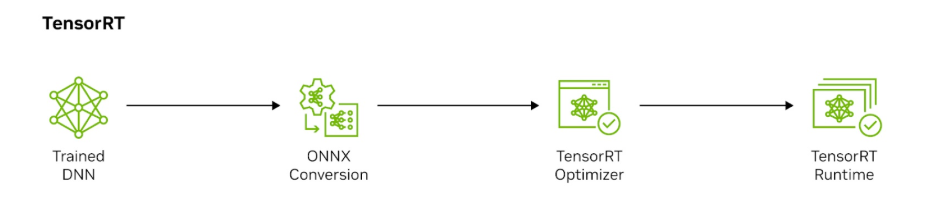
\includegraphics[width=0.8\textwidth]{images/estado_del_arte/TensorRT_pipeline.png}
   \caption{Ejemplo de flujo de trabajo de optimización con TensorRT.}
   \label{fig:tensorrt_architecture}
\end{figure}

El proceso de optimización con TensorRT, como se ilustra en la Figura~\ref{fig:tensorrt_architecture}, genera un motor de inferencia ajustado para el hardware NVIDIA subyacente, seleccionando las rutas de ejecución más eficientes. TensorRT se integra con los principales frameworks de aprendizaje profundo, como TensorFlow, PyTorch y ONNX, facilitando la importación de modelos para su optimización.



\section{Seguimiento de objetos en tiempo real}
En esta sección se presentará los conceptos básicos del seguimiento de objetos en tiempo real, se explicará el problema del seguimiento de objetos múltiples (MOT) y se presentarán los algoritmos más relevantes en este campo.

\subsection{Introducción al seguimiento de objetos}
El seguimiento de objetos es un proceso que complementa la salida de los modelos de detección. Mientras que un modelo de detección opera sobre cada fotograma de forma independiente, identificando y localizando objetos como si fueran imágenes estáticas, el Seguimiento de Objetos Múltiples (MOT) actúa sobre estas detecciones para establecer una correspondencia temporal. La función esencial del MOT es asignar un identificador único a cada objeto detectado en un fotograma y mantener dicho identificador de manera consistente a lo largo de la secuencia de vídeo. Esto permite reconstruir las trayectorias de los objetos y analizar su comportamiento dinámico en la escena.

Para realizar este seguimiento, el MOT se basa en la información temporal y espacial de las detecciones. Utiliza técnicas de predicción y asociación para determinar la continuidad de los objetos a lo largo del tiempo, teniendo en cuenta factores como la posición, velocidad y apariencia de los objetos. El algoritmo utilizado para el seguimiento puede variar en complejidad, desde enfoques simples que utilizan filtros de Kalman para predecir la posición futura de un objeto, hasta métodos más avanzados que incorporan redes neuronales profundas para aprender características de apariencia y mejorar la robustez del seguimiento.


El filtro de Kalman es un algoritmo de estimación recursivo fundamental en el seguimiento de objetos. Funciona como un estimador óptimo para sistemas dinámicos lineales, permitiendo predecir el estado futuro de un objeto (como su posición y velocidad) a partir de una serie de mediciones ruidosas o incompletas a lo largo del tiempo. Su proceso se basa en dos etapas cíclicas:
\begin{itemize}
   \item \textbf{Predicción:} Utiliza un modelo dinámico del movimiento esperado del objeto para estimar su estado en el siguiente instante de tiempo.
   \item \textbf{Actualización:} Incorpora la nueva medición (detección) obtenida en ese instante para corregir la predicción inicial, ponderando la información del modelo y la medición según su incertidumbre asociada.
\end{itemize}
Este ciclo permite al filtro refinar continuamente la estimación del estado del objeto, suavizar las trayectorias y manejar eficazmente el ruido inherente a las mediciones del detector. Es una herramienta clave para mantener la identidad de los objetos entre fotogramas, especialmente cuando las detecciones son intermitentes o imprecisas.



\begin{figure}[H]
   \centering
   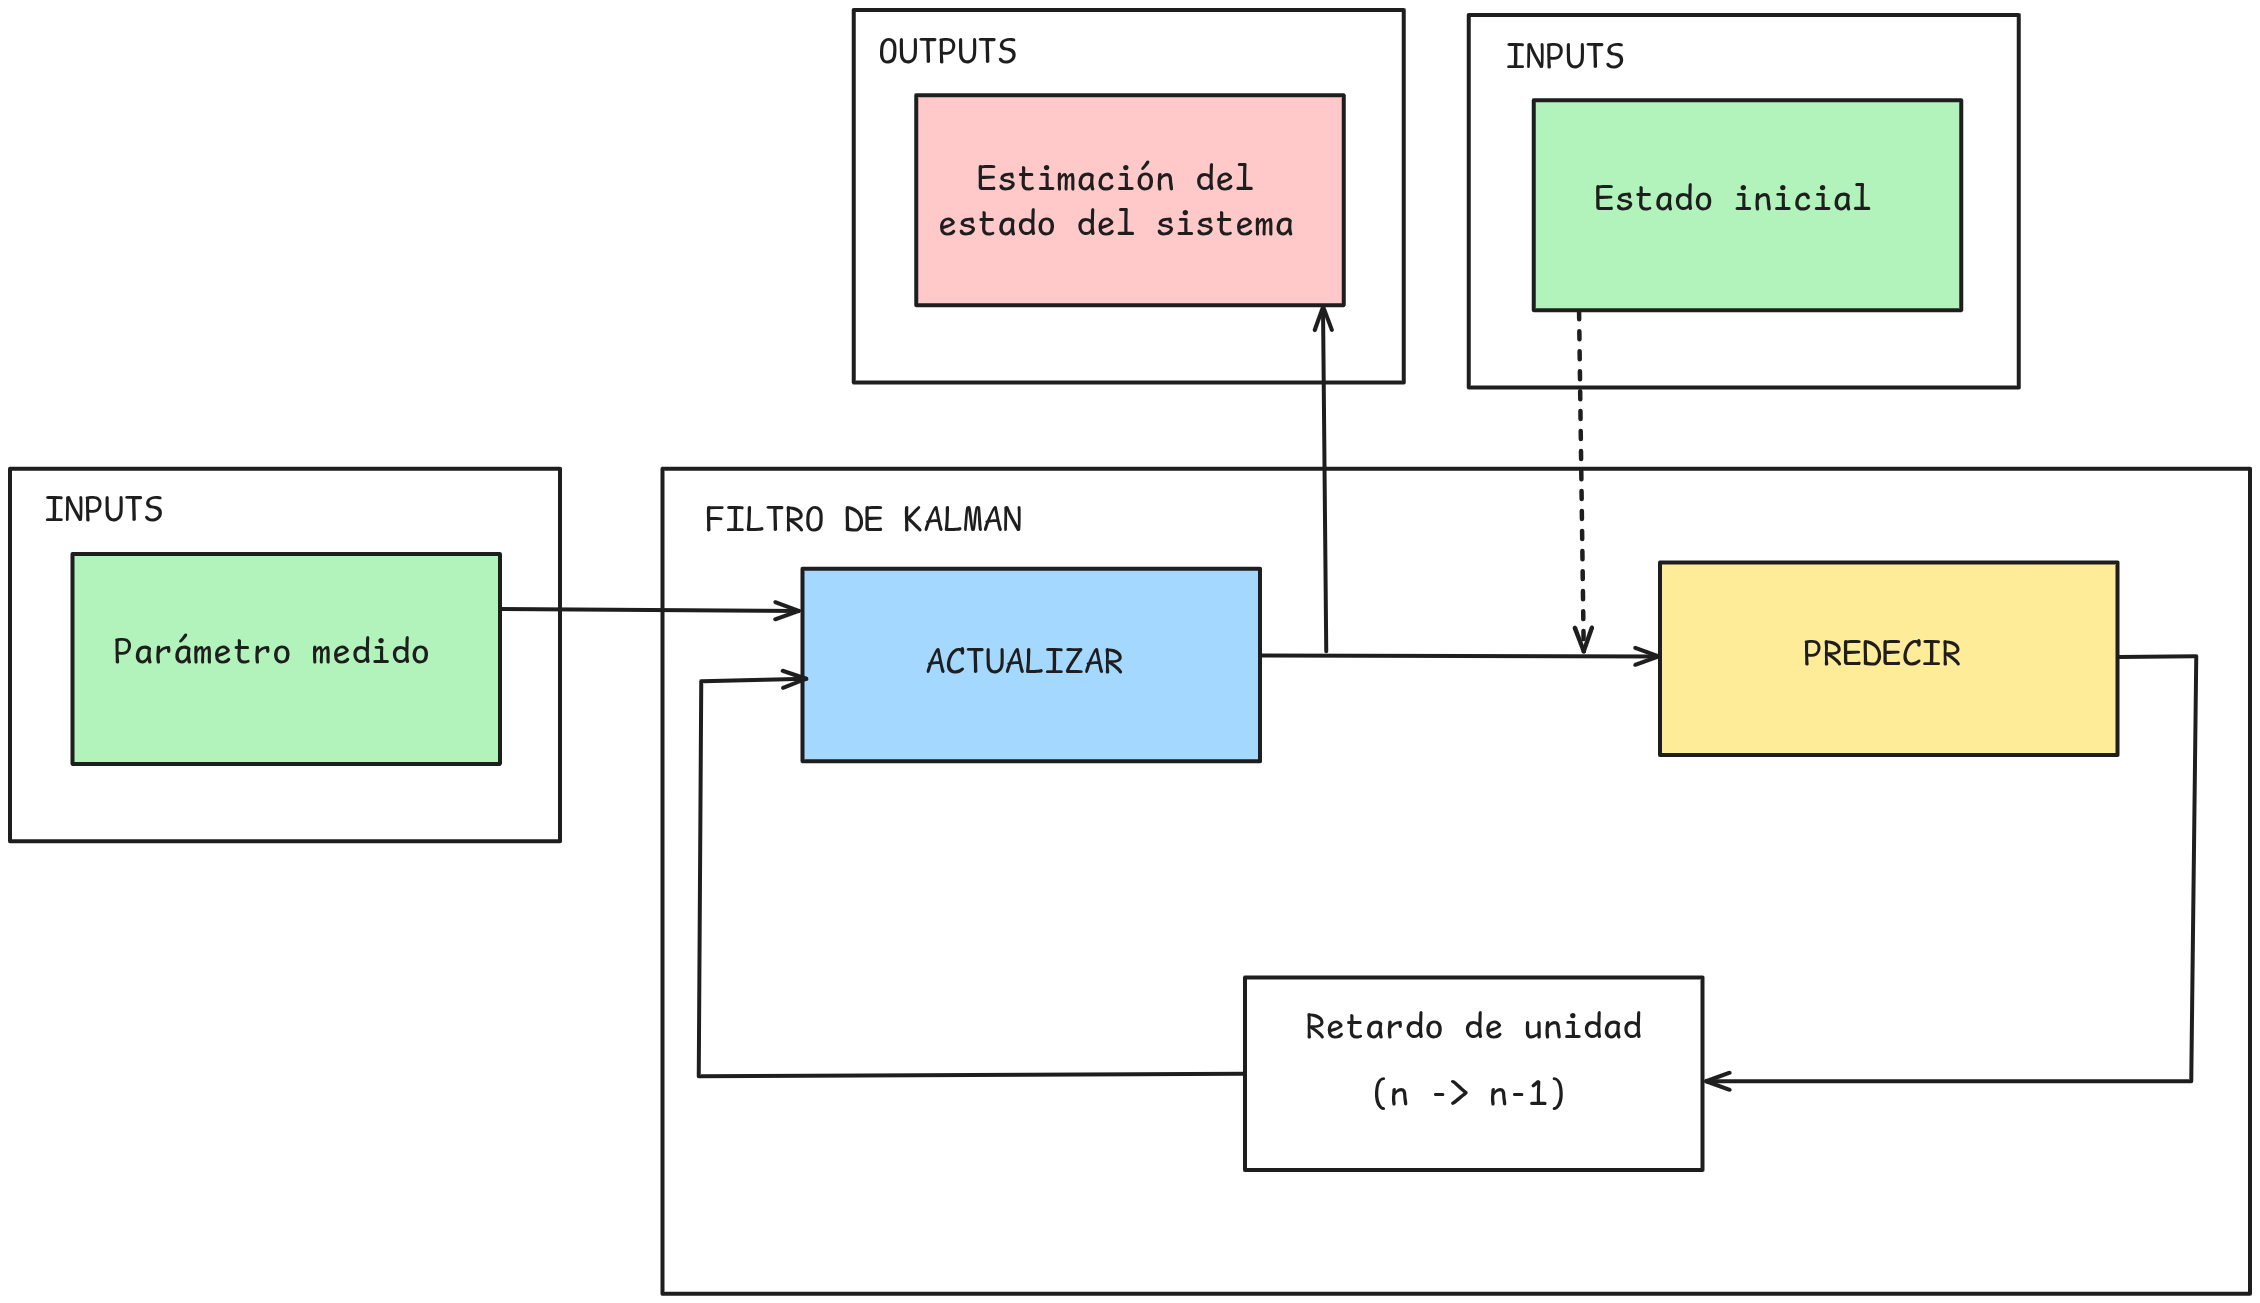
\includegraphics[width=0.8\textwidth]{images/estado_del_arte/filtro_de_kalman.png}
   \caption{Diagrama de flujo del filtro de Kalman.}
   \label{fig:filtro_de_kalman}
\end{figure}

La Figura ~\ref{fig:filtro_de_kalman} representa el funcionamiento de un filtro de Kalman, un algoritmo muy utilizado para estimar el estado de un sistema dinámico en presencia de ruido e incertidumbre. A continuación se explica cada bloque:

\begin{itemize}
   \item \textbf{INPUTS: Parámetro medido}
   Este bloque representa las mediciones que se obtienen del sistema. Estas mediciones contienen errores (ruido), por lo que no se usan directamente, sino que se pasan al filtro para su procesamiento.

   \item \textbf{INPUTS: Estado inicial}
   Proporciona una estimación inicial del estado del sistema y su incertidumbre asociada. Esta información se utiliza para arrancar el filtro de Kalman.

   \item \textbf{ACTUALIZAR}
   Este es uno de los dos pasos principales del filtro de Kalman. Combina la predicción previa con la medición actual para actualizar la estimación del estado del sistema y ajusta la incertidumbre de esa estimación.

   \item \textbf{PREDECIR}
   El otro paso clave del filtro utiliza el modelo del sistema para predecir el siguiente estado y su incertidumbre, basándose en la estimación anterior y considerando el retardo de una unidad.

   \item \textbf{Retardo de unidad (\(n \rightarrow n{-}1\))}
   Este bloque representa el almacenamiento del estado estimado en el instante anterior para ser utilizado en la siguiente predicción.

   \item \textbf{OUTPUTS: Estimación del estado del sistema}
   Este es el resultado final del filtro: una estimación refinada del estado actual del sistema, que es más precisa que la simple medición directa.
\end{itemize}

En conjunto, el filtro de Kalman realiza un ciclo continuo de predicción y corrección, usando tanto el modelo del sistema como las mediciones reales, para obtener una estimación óptima del estado.



% \begin{itemize}
%    \item \textbf{Introducción al Seguimiento de Objetos Múltiples (MOT):} Definición del problema, importancia y aplicaciones principales.
%    \item \textbf{Desafíos del MOT:} Se discutirán las dificultades inherentes al seguimiento, como oclusiones, cambios de apariencia, interacciones entre objetos, entradas y salidas de la escena, y errores de detección.
%    \item \textbf{Paradigma Tracking-by-Detection:} Explicación del enfoque dominante en MOT, que consiste en detectar objetos en cada fotograma y luego asociar estas detecciones a lo largo del tiempo para formar trayectorias.
%    \item \textbf{Filtro de Kalman:} Descripción de sus fundamentos matemáticos como estimador óptimo para sistemas lineales y su aplicación para predecir la posición futura de los objetos y suavizar las trayectorias, manejando la incertidumbre en las mediciones.
%    \item \textbf{Asociación de Datos:} Técnicas para vincular las detecciones actuales con las trayectorias existentes, como el algoritmo Húngaro basado en métricas de similitud (IoU, apariencia).
%    \item \textbf{Algoritmos Clásicos:}
%       \begin{itemize}
%          \item \textbf{SORT (Simple Online and Realtime Tracking):} Enfoque basado principalmente en el Filtro de Kalman y la métrica IoU para la asociación, destacando por su simplicidad y velocidad.
%          \item \textbf{DeepSORT (Deep Simple Online and Realtime Tracking):} Extensión de SORT que incorpora características de apariencia extraídas mediante redes profundas para mejorar la robustez frente a oclusiones prolongadas.
%       \end{itemize}
%    \item \textbf{Algoritmos Modernos - BYTETrack:} Presentación de BYTETrack, que mejora la gestión de detecciones de baja confianza para manejar mejor las oclusiones y reducir la fragmentación de trayectorias, separando las detecciones de alta y baja confianza en el proceso de asociación.
%    \item \textbf{Métricas de Evaluación para MOT:} Introducción a las métricas estándar para evaluar el rendimiento de los algoritmos de seguimiento, como MOTA (Multiple Object Tracking Accuracy), MOTP (Multiple Object Tracking Precision), IDF1, HOTA (Higher Order Tracking Accuracy), entre otras.
% \end{itemize}


\subsection{BYTETrack}

BYTETrack \cite{zhang2022bytetrackmultiobjecttrackingassociating} es un algoritmo avanzado de Seguimiento de Objetos Múltiples (MOT) que se inscribe dentro del paradigma de seguimiento por detección (\textit{tracking-by-detection}). Este paradigma consiste en detectar objetos en cada fotograma de forma independiente y luego asociar estas detecciones a lo largo del tiempo para construir trayectorias coherentes. La innovación fundamental de BYTETrack reside en su novedoso método de asociación de datos, denominado BYTE, que aborda explícitamente un problema común en MOT: el manejo de detecciones con baja puntuación de confianza.

Mientras que la mayoría de los algoritmos de seguimiento descartan las detecciones por debajo de un cierto umbral de confianza para evitar la introducción de falsos positivos, BYTETrack reconoce que estas detecciones de baja confianza a menudo corresponden a objetos reales que están parcialmente ocluidos o cuya apariencia ha cambiado temporalmente. Descartarlas puede llevar a la pérdida de trayectorias y a una menor precisión general del seguimiento. Esta estrategia de asociación en dos pasos permite a BYTETrack recuperar objetos reales incluso cuando la confianza del detector disminuye debido a oclusiones o desenfoque, manteniendo la continuidad de las trayectorias. Al separar claramente las detecciones de alta y baja confianza y utilizarlas de manera diferenciada en el proceso de asociación, BYTETrack logra una notable mejora en la robustez del seguimiento, reduce significativamente la fragmentación de las trayectorias (medida por métricas como IDF1) y maneja eficazmente las variaciones en la calidad de las detecciones, todo ello manteniendo una alta eficiencia computacional.

\begin{figure}[H]
   \centering
   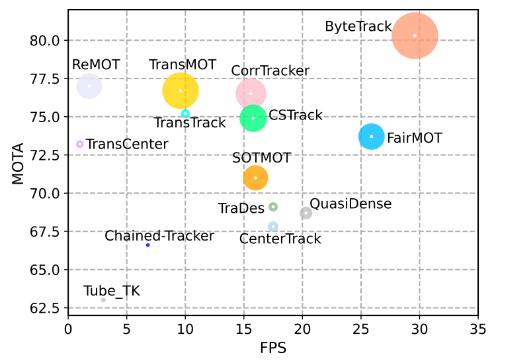
\includegraphics[width=0.5\textwidth]{images/estado_del_arte/BYTETrack_MOTA.png}
   \caption{Comparativa de rendimiento de BYTETrack con otros algoritmos de seguimiento.}
   \label{fig:bytetrack_mota}
\end{figure}

La Figura \ref{fig:bytetrack_mota} presenta una comparativa de rendimiento que evidencia la superioridad de BYTETrack frente a otros algoritmos de seguimiento, según los resultados publicados en \cite{zhang2022bytetrackmultiobjecttrackingassociating}. Como se observa, BYTETrack no solo alcanza una mayor precisión, medida por la métrica MOTA (Multiple Object Tracking Accuracy), sino que también demuestra una velocidad de procesamiento superior. Estas características lo posicionan como una solución particularmente eficaz y atractiva para aplicaciones que demandan seguimiento de objetos en tiempo real.

\begin{figure}[H]

   \centering
   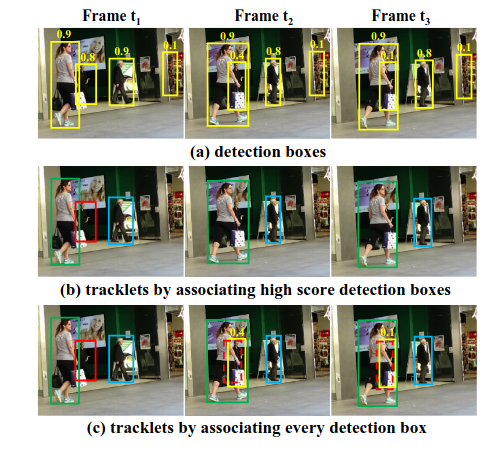
\includegraphics[width=0.5\textwidth]{images/estado_del_arte/BYTETrack_deteccion.png}
   \caption{Ejemplo de detección y seguimiento de objetos utilizando BYTETrack.}
   \label{fig:bytetrack_deteccion}
   \caption*{Fuente: \cite{zhang2022bytetrackmultiobjecttrackingassociating}}
\end{figure}

La Figura \ref{fig:bytetrack_deteccion} ilustra el proceso de BYTETrack a través de tres fotogramas consecutivos ($\tau_1$, $\tau_2$, $\tau_3$) de una secuencia de vídeo. En (a), se observan las detecciones iniciales que superan un umbral de confianza (p. ej., 0.5). La sección (b) muestra las trayectorias generadas al asociar exclusivamente las detecciones de alta confianza. Por el contrario, (c) presenta el resultado final de BYTETrack, que integra también las detecciones de baja confianza en el proceso de asociación. Esta comparación evidencia cómo la estrategia de BYTETrack permite mantener la continuidad de las trayectorias frente a desafíos como oclusiones parciales y variaciones en la confianza de las detecciones, logrando así una representación más precisa y robusta del movimiento de los objetos en el tiempo.



El funcionamiento del algoritmo BYTETrack es el siguiente:

\textbf{Input:} Una secuencia de vídeo $V$, un detector de objetos $Det$, y un umbral de confianza de detección $\tau$.

\textbf{Output:} Las trayectorias $\mathcal{T}$ de los objetos detectados en el vídeo.

\begin{enumerate}
   \item \textbf{Inicialización:} Se inicializa el conjunto de trayectorias $\mathcal{T}$ como vacío.
   \item \textbf{Procesamiento por fotograma:} Para cada fotograma $f_k$ en la secuencia de vídeo $V$:
   { % Start a group to keep the redefinition local
   \renewcommand{\theenumii}{\theenumi.\arabic{enumii}} % Change numbering to 1.1, 1.2, etc.
   \renewcommand{\labelenumii}{\theenumii.} % Add trailing dot to the label
   \begin{enumerate}
      \item \textbf{Detección:} Se utiliza el detector $Det$ para obtener las cajas delimitadoras y sus puntuaciones de confianza para el fotograma $f_k$, resultando en un conjunto de detecciones $\mathcal{D}_k$.
      \item \textbf{Separación de detecciones:} Se inicializan dos conjuntos vacíos: $\mathcal{D}_{high}$ para detecciones de alta confianza y $\mathcal{D}_{low}$ para detecciones de baja confianza. Se itera sobre cada detección $d$ en $\mathcal{D}_k$:
      \begin{itemize}
         \item Si la puntuación $d.score$ es mayor que el umbral $\tau$, la detección $d$ se añade a $\mathcal{D}_{high}$.
         \item En caso contrario, la detección $d$ se añade a $\mathcal{D}_{low}$.
      \end{itemize}
      \item \textbf{Predicción de trayectorias:} Para cada trayectoria existente $t$ en $\mathcal{T}$, se predice su nueva ubicación utilizando un Filtro de Kalman.
      \item \textbf{Primera asociación:} Se asocian las trayectorias $\mathcal{T}$ con las detecciones de alta confianza $\mathcal{D}_{high}$ utilizando el \textit{Hungarian alogorithm}\cite{kuhn1955hungarian} con la métrica de similitud IoU (Intersection over Union). Las detecciones no asociadas se guardan en $\mathcal{D}_{remain}$ y las trayectorias no asociadas en $\mathcal{T}_{remain}$.
      \item \textbf{Segunda asociación:} Se asocian las trayectorias restantes $\mathcal{T}_{remain}$ con las detecciones de baja confianza $\mathcal{D}_{low}$ utilizando otra métrica de similitud (Similarity\#2, usualmente IoU). Las trayectorias que siguen sin asociarse se guardan en $\mathcal{T}_{re-remain}$. Solo se asocian detecciones de baja confianza a trayectorias que no pudieron ser asociadas con detecciones de alta confianza.
      \item \textbf{Eliminación de trayectorias no asociadas:} Se eliminan de $\mathcal{T}$ las trayectorias que quedaron en $\mathcal{T}_{re-remain}$ (aquellas que no se pudieron asociar ni en la primera ni en la segunda etapa) si han permanecido sin asociar durante un número determinado de fotogramas (definido por el parámetro track\_buffer).
      \item \textbf{Inicialización de nuevas trayectorias:} Se itera sobre las detecciones de alta confianza que no fueron asociadas ($\mathcal{D}_{remain}$). Cada una de estas detecciones se considera el inicio de una nueva trayectoria y se añade al conjunto $\mathcal{T}$.
   \end{enumerate}
   } % End the group
   \item \textbf{Retorno:} Una vez procesados todos los fotogramas, se devuelve el conjunto final de trayectorias $\mathcal{T}$.
\end{enumerate}




\section{Slicing Aided Hyper Inference}
Explicación de la técnica de Slicing Aided Hyper Inference, como se utiliza para mejorar la precisión de los modelos de detección de objetos y como se aplica en este trabajo.

\chapter{Análisis del problema}

????? ????????????? ????????????? ????????????? ????????????? ????????????? 

\chapter{Diseño e implementación de la solución}
En este capítulo se explicará la solución propuesta, como se ha diseñado y como se ha implementado.

\section{Descripción del sistema}

Descripción del sistema de visión artificial propuesto, como se ha diseñado y como se ha implementado.

\section{Diseño de las etapas del sistema}

Descripción de las etapas del sistema, como se han diseñado y como se han implementado.

Etapas del sistema:
\begin{itemize}
   \item \textbf{Captura de imágenes:} Descripción de la etapa de captura de imágenes, como se ha diseñado y como se ha implementado.
   \item \textbf{Inferencia:} Descripción de la etapa de inferencia, como se ha diseñado y como se ha implementado.
   \item \textbf{Seguimiento:} Descripción de la etapa de seguimiento, como se ha diseñado y como se ha implementado.
   \item \textbf{Escritura de resultados:} Descripción de la etapa de escritura de resultados, como se ha diseñado y como se ha implementado.
\end{itemize}

\section{Segmentación de las etapas del sistema}

Tipos de segmentación de las etapas del sistema:

\begin{itemize}
   \item \textbf{No segmentada:} Secuencial
   \item \textbf{Segmentación basada en hilos:} Cada etapa del sistema se ejecuta en un hilo diferente.
   \item \textbf{Segmentación basada en procesos:} Cada etapa del sistema se ejecuta en un proceso diferente.
   \item \textbf{Segmentación basada en hardware:} La etapa de inferencia se ejecuta en GPU, DLA0 y DLA1.
   \item \textbf{Segmentación basada en procesos con memoria compartida:} Cada etapa del sistema se ejecuta en un proceso diferente, pero comparten la memoria.
\end{itemize}
    


\chapter{Análisis de la solución}

En este capítulo se analizará la solución propuesta variando los parámetros posibles

\section{Variación de los parámetros}
Explicación de los parámetros que se pueden variar en la solución propuesta y su efecto en el rendimiento del sistema.

------PRUEBA--------


\begin{table}[h]
   \centering
   \resizebox{\textwidth}{!}{ % Ajusta el ancho al tamaño de la página
   \pgfplotstabletypeset[
       col sep=comma, % Definir separador de columnas (por si el CSV usa comas)
       header=true,    % Usar la primera línea como encabezado
       columns={Model, IoU, CPU_Inference, GPU_Inference, DLA_Inference, CPU_Power, GPU_Power, DLA_Power, CPU_Energy, GPU_Energy, DLA_Energy}, % Seleccionar columnas a mostrar
       display columns/0/.style={column name=Model, string type}, % Formato de la columna 'Model'
       display columns/1/.style={column name=IoU}, % Formato de la columna 'IoU'
       display columns/2/.style={column name=CPU\_Inference, column type={|c|}}, % Estilo para columnas de inferencia
       display columns/3/.style={column name=GPU\_Inference, column type={|c|}}, 
       display columns/4/.style={column name=DLA\_Inference, column type={|c|}},
       display columns/5/.style={column name=CPU\_Power, column type={|c|}}, % Estilo para columnas de potencia
       display columns/6/.style={column name=GPU\_Power, column type={|c|}},
       display columns/7/.style={column name=DLA\_Power, column type={|c|}},
       display columns/8/.style={column name=CPU\_Energy, column type={|c|}}, % Estilo para columnas de energía
       display columns/9/.style={column name=GPU\_Energy, column type={|c|}},
       display columns/10/.style={column name=DLA\_Energy, column type={|c|}},
       every head row/.style={before row=\toprule, after row=\midrule}, % Reglas horizontales en el encabezado
       every last row/.style={after row=\bottomrule}, % Reglas horizontales al final
       every column/.style={sci zerofill}, % Opcional, ajusta el formato numérico
       empty cells with={NaN} % Reemplaza celdas vacías o con guiones por NaN
   ]{excels/model_comparasion.csv} % Aquí pones la ruta del archivo CSV
   }
   \caption{Comparación de modelos en términos de inferencia, consumo de energía y potencia.}
   \label{tab:model_comparasion}
\end{table}



------PRUEBA--------



\section{Tipo de segmentación}
En esta sección se analizará el rendimiento de la solución propuesta variando el tipo de segmentación de las etapas del sistema con gráficas y tablas.

\section{Talla del modelo}
En esta sección se analizará el rendimiento de la solución propuesta variando la talla del modelo de detección de objetos con gráficas y tablas.

\section{Precisión del modelo}
En esta sección se analizará el rendimiento de la solución propuesta variando la precisión del modelo de detección de objetos con gráficas y tablas.

\section{Modo de energía y cores de la CPU}
En esta sección se analizará el rendimiento de la solución propuesta variando el modo de energía del dispositivo y el número de cores de la CPU con gráficas y tablas.

\section{Tamaño de la imagen}
En esta sección se analizará el rendimiento de la solución propuesta variando el tamaño de la imagen de entrada del modelo con la técnica de Slicing Aided Hyper Inference (SAHI) con gráficas y tablas.

\chapter{Prueba de concepto}
Aqui se explicará la implementación de la solución propuesta en el entorno de producción con la cinta transportadora.

\section{Construcción del entorno}

\section{Instalación del entorno}






????? ????????????? ????????????? ????????????? ????????????? ?????????????


%%%%%%%%%%%%%%%%%%%%%%%%%%%%%%%%%%%%%%%%%%%%%%%%%%%%%%%%%%%%%%%%%%%%%%%%%%%%%%%
%                                 CONCLUSIONS                                 %
%%%%%%%%%%%%%%%%%%%%%%%%%%%%%%%%%%%%%%%%%%%%%%%%%%%%%%%%%%%%%%%%%%%%%%%%%%%%%%%

\chapter{Conclusiones}

????? ????????????? ????????????? ????????????? ????????????? ????????????? 

%%%%%%%%%%%%%%%%%%%%%%%%%%%%%%%%%%%%%%%%%%%%%%%%%%%%%%%%%%%%%%%%%%%%%%%%%%%%%%%
%                                BIBLIOGRAFIA                                 %
%%%%%%%%%%%%%%%%%%%%%%%%%%%%%%%%%%%%%%%%%%%%%%%%%%%%%%%%%%%%%%%%%%%%%%%%%%%%%%%

\printglossaries


\bibliographystyle{plain}      % Estilo de la bibliografía
\bibliography{referencias} % Bibliografia

% \begin{thebibliography}{10}

% %%%%%%%%%%%%%%%%%%%%%%%%%%%%%%%%%%%%%%%%%%%%%%%%%%%%%%%%%%%%%%%%%%%%%%%%%%%%%%%
% % MODEL D'ARTICLE                                                             %
% %%%%%%%%%%%%%%%%%%%%%%%%%%%%%%%%%%%%%%%%%%%%%%%%%%%%%%%%%%%%%%%%%%%%%%%%%%%%%%%
% \bibitem{light}
%    Jennifer~S. Light.
%    \newblock When computers were women.
%    \newblock \textit{Technology and Culture}, 40:3:455--483, juliol, 1999.

% %%%%%%%%%%%%%%%%%%%%%%%%%%%%%%%%%%%%%%%%%%%%%%%%%%%%%%%%%%%%%%%%%%%%%%%%%%%%%%%
% % MODEL DE LLIBRE                                                             %
% %%%%%%%%%%%%%%%%%%%%%%%%%%%%%%%%%%%%%%%%%%%%%%%%%%%%%%%%%%%%%%%%%%%%%%%%%%%%%%%
% \bibitem{ifrah}
%    Georges Ifrah.
%    \newblock \textit{Historia universal de las cifras}.
%    \newblock Espasa Calpe, S.A., Madrid, sisena edició, 2008.

% %%%%%%%%%%%%%%%%%%%%%%%%%%%%%%%%%%%%%%%%%%%%%%%%%%%%%%%%%%%%%%%%%%%%%%%%%%%%%%%
% % MODEL D'URL                                                                 %
% %%%%%%%%%%%%%%%%%%%%%%%%%%%%%%%%%%%%%%%%%%%%%%%%%%%%%%%%%%%%%%%%%%%%%%%%%%%%%%%
% \bibitem{WAR}
% Comunicat de premsa del Departament de la Guerra, 
% emés el 16 de febrer de 1946. 
% \newblock Consultat a 
% \url{http://americanhistory.si.edu/comphist/pr1.pdf}.

% \end{thebibliography}
\cleardoublepage

%%%%%%%%%%%%%%%%%%%%%%%%%%%%%%%%%%%%%%%%%%%%%%%%%%%%%%%%%%%%%%%%%%%%%%%%%%%%%%%
%                           APÈNDIXS  (Si n'hi ha!)                           %
%%%%%%%%%%%%%%%%%%%%%%%%%%%%%%%%%%%%%%%%%%%%%%%%%%%%%%%%%%%%%%%%%%%%%%%%%%%%%%%

\APPENDIX

%%%%%%%%%%%%%%%%%%%%%%%%%%%%%%%%%%%%%%%%%%%%%%%%%%%%%%%%%%%%%%%%%%%%%%%%%%%%%%%
%                         LA CONFIGURACIO DEL SISTEMA                         %
%%%%%%%%%%%%%%%%%%%%%%%%%%%%%%%%%%%%%%%%%%%%%%%%%%%%%%%%%%%%%%%%%%%%%%%%%%%%%%%




\chapter{Configuración del sistema}

????? ????????????? ????????????? ????????????? ????????????? ?????????????

\section{Fase de inicialitzación}

????? ????????????? ????????????? ????????????? ????????????? ?????????????

\section{Identificación de dispositivos}

????? ????????????? ????????????? ????????????? ????????????? ?????????????

%%%%%%%%%%%%%%%%%%%%%%%%%%%%%%%%%%%%%%%%%%%%%%%%%%%%%%%%%%%%%%%%%%%%%%%%%%%%%%%
%                               ALTRES  APÈNDIXS                              %
%%%%%%%%%%%%%%%%%%%%%%%%%%%%%%%%%%%%%%%%%%%%%%%%%%%%%%%%%%%%%%%%%%%%%%%%%%%%%%%


\chapter{Objetivos de Desarrollo Sostenible}

\begin{tabularx}{\textwidth}{|>{\raggedright\arraybackslash}X|c|c|c|c|}\hline
   \textbf{Objetivos de Desarrollo Sostenible} & \textbf{Alto} & \textbf{Medio} & \textbf{Bajo} & \textbf{No procede} \\ \hline
   ODS 1.  \textbf{Fin de la pobreza.}                            & & & & X \\ \hline
   ODS 2.  \textbf{Hambre cero.}                                  & & X & & \\ \hline
   ODS 3.  \textbf{Salud y bienestar.}                            & & & & X\\ \hline
   ODS 4.  \textbf{Educaci\'on de calidad.}                       & & & & X \\ \hline
   ODS 5.  \textbf{Igualdad de g\'enero.}                         & & & & X \\ \hline
   ODS 6.  \textbf{Agua limpia y saneamiento.}                    & & & & X \\ \hline
   ODS 7.  \textbf{Energ\'{\i}a asequible y no contaminante.}     & & & & X\\ \hline
   ODS 8.  \textbf{Trabajo decente y crecimiento econ\'omico.}    & X & & & \\ \hline
   ODS 9.  \textbf{Industria, innovaci\'on e infraestructuras.}   & X & & & \\ \hline
   ODS 10. \textbf{Reducci\'on de las desigualdades.}             & & & & X\\ \hline
   ODS 11. \textbf{Ciudades y comunidades sostenibles.}           & & & & X\\ \hline
   ODS 12. \textbf{Producci\'on y consumo responsables.}          & X & & & \\ \hline
   ODS 13. \textbf{Acci\'on por el clima.}                        & & & X & \\ \hline
   ODS 14. \textbf{Vida submarina.}                               & & & & X \\ \hline
   ODS 15. \textbf{Vida de ecosistemas terrestres.}               & & & & X\\ \hline
   ODS 16. \textbf{Paz, justicia e instituciones s\'olidas.}      & & & & X\\ \hline
   ODS 17. \textbf{Alianzas para lograr objetivos.}               & & & & X\\ \hline
   \end{tabularx}


   \section*{Justificación de los Objetivos de Desarrollo Sostenible}

   \textbf{ODS-8. Trabajo decente y crecimiento económico:} Este proyecto contribuye directamente al crecimiento económico sostenible mediante la automatización inteligente de procesos de control de calidad. La implementación de sistemas de detección de defectos basados en IA permite reducir costes operativos, minimizar desperdicios y optimizar la cadena de producción, lo que se traduce en mayor productividad y competitividad empresarial. Se alinea específicamente con la meta 8.2 de la ONU: «Lograr niveles más elevados de productividad económica mediante la diversificación, la modernización tecnológica y la innovación», al incorporar tecnologías avanzadas de procesamiento de imágenes y aprendizaje automático en entornos industriales tradicionales.

   \textbf{ODS-9. Industria, innovación e infraestructura:} El desarrollo de sistemas inteligentes para la detección de defectos representa una clara apuesta por la innovación industrial. Este proyecto no solo implementa tecnologías emergentes como la IA en procesos productivos, sino que además optimiza su rendimiento mediante el uso eficiente de hardware especializado como GPUs, algoritmos de seguimiento multi-objeto y técnicas de paralelización. Esto responde directamente a la meta 9.4 de la ONU: «Modernizar la infraestructura y reconvertir las industrias para que sean sostenibles, utilizando los recursos con mayor eficacia y promoviendo la adopción de tecnologías y procesos industriales limpios y ambientalmente racionales», al permitir mejoras significativas en eficiencia energética y uso de recursos mediante sistemas de inspección automatizados.

   \textbf{ODS-12. Producción y consumo responsables:} La implementación de sistemas de detección temprana de defectos contribuye sustancialmente a la producción responsable mediante: 1) la reducción del descarte de productos y materias primas al identificar problemas en etapas iniciales del proceso productivo, 2) la optimización del consumo energético al evitar el procesamiento completo de productos defectuosos, y 3) la mejora de la calidad final que aumenta la vida útil de los productos. Estas aportaciones se vinculan directamente con la meta 12.5 de la ONU: «De aquí a 2030, reducir considerablemente la generación de desechos mediante actividades de prevención, reducción, reciclado y reutilización», ya que el sistema desarrollado actúa preventivamente evitando la generación de residuos industriales y facilitando la reutilización de materiales recuperados.

%%%%%%%%%%%%%%%%%%%%%%%%%%%%%%%%%%%%%%%%%%%%%%%%%%%%%%%%%%%%%%%%%%%%%%%%%%%%%%%
%                              FI DEL DOCUMENT                                %
%%%%%%%%%%%%%%%%%%%%%%%%%%%%%%%%%%%%%%%%%%%%%%%%%%%%%%%%%%%%%%%%%%%%%%%%%%%%%%%

\end{document}
